\documentclass[11pt,nswissgerman]{article}
\usepackage{helvet}
\renewcommand{\familydefault}{\sfdefault}
\usepackage[latin2]{inputenc}
\usepackage{textcomp}
\usepackage[a4paper]{geometry}
\geometry{verbose,tmargin=3cm,bmargin=3cm,lmargin=3.5cm,rmargin=3.5cm,headheight=3cm,headsep=1cm,footskip=2cm}
\usepackage{fancyhdr}
\pagestyle{fancy}
\usepackage{wrapfig}
\usepackage{graphicx}
\usepackage[position=bottom]{subfig}
\usepackage{titletoc}
\usepackage{float}
\makeatletter
\@ifundefined{date}{}{\date{}}
\makeatother
\usepackage{babel}
\usepackage[
            colorlinks=true,
            urlcolor=green,
            linkcolor=black
]{hyperref}
\setcounter{secnumdepth}{1} % levels under \section are not numbered
\setcounter{tocdepth}{2}    % levels under \subsection are not listed in the TOC
\begin{document}
\author{Stefan Bopp}
\title{\Huge Reise nach Sardinien 2013\vspace{2cm}

\includegraphics[width=0.4\textwidth]{../Bilder/Logo/Logo.png}
}
\maketitle
\vfill
\tableofcontents

\newpage

\lhead{Sardinien 2013}

\rhead{jackthebus.com}

\cfoot{\thepage}
%\begin{wrapfigure}{R}{0.45\textwidth} 
%  \begin{centering}
%    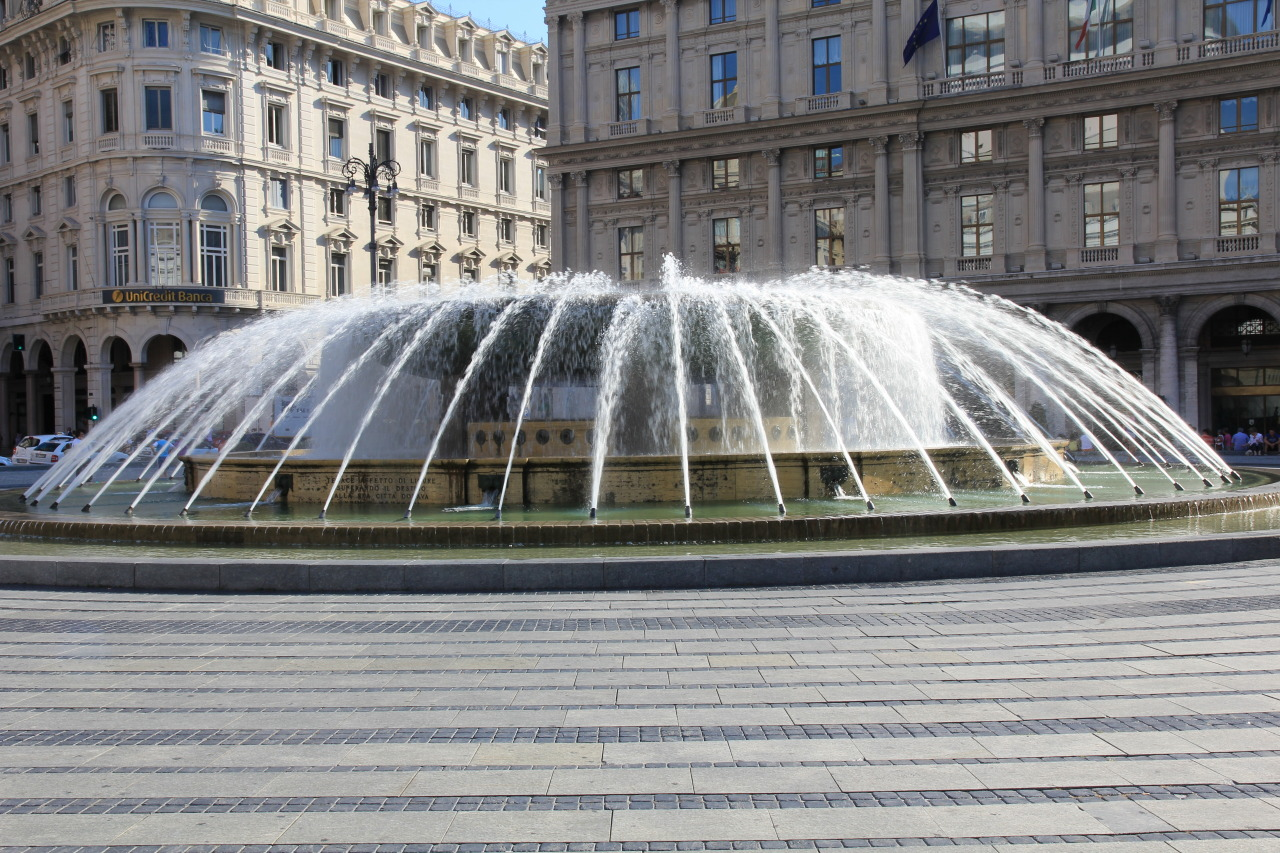
\includegraphics[width=0.4\textwidth, height=5cm, keepaspectratio]{../Bilder/Sardinien/1.jpg}
%    \caption{Regen}
%  \end{centering}
%\end{wrapfigure} 

%\begin{figure}[b]
%   \centering
%      %\subfloat[CAPTION]{BILDERCODE}\qquad
%   \subfloat{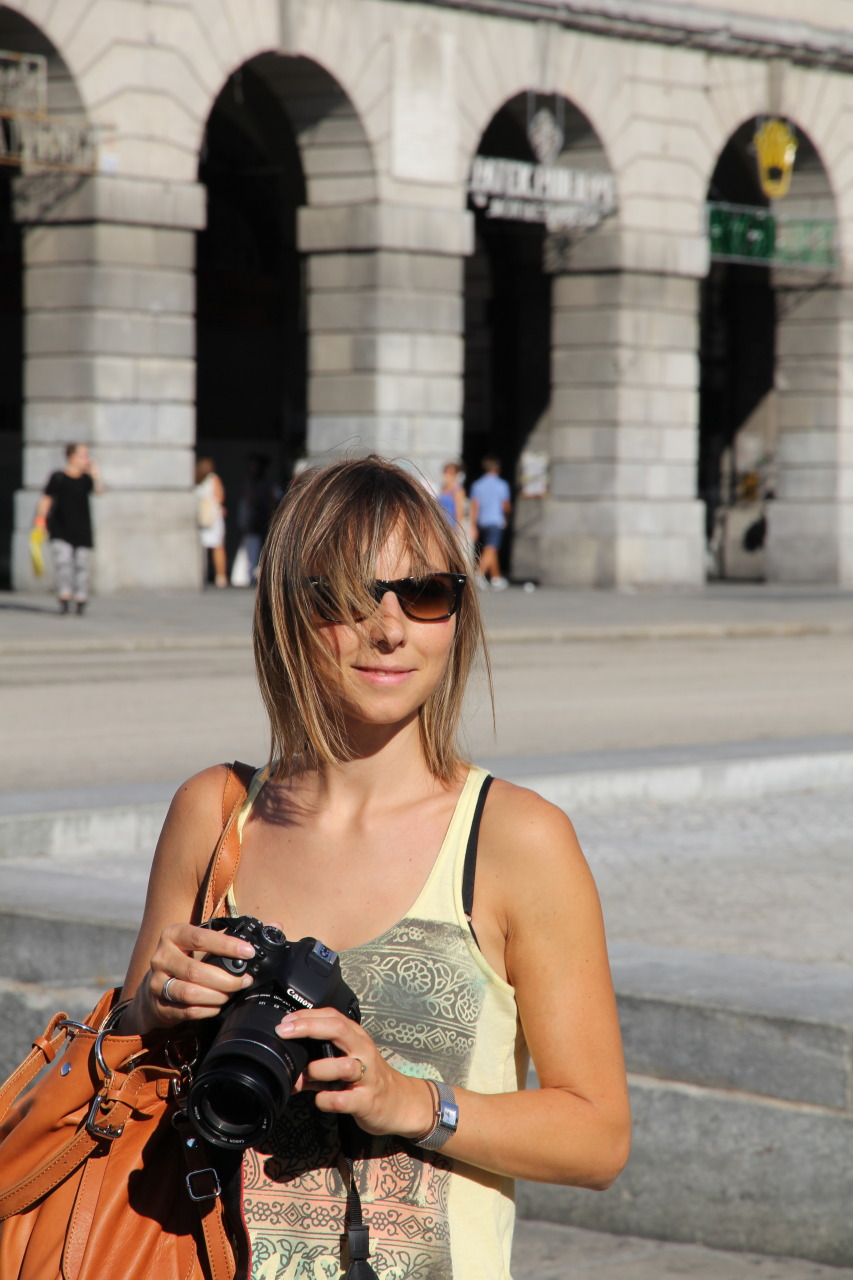
\includegraphics [width=0.3\textwidth]{../Bilder/Sardinien/2.jpg}}\quad
%   \subfloat{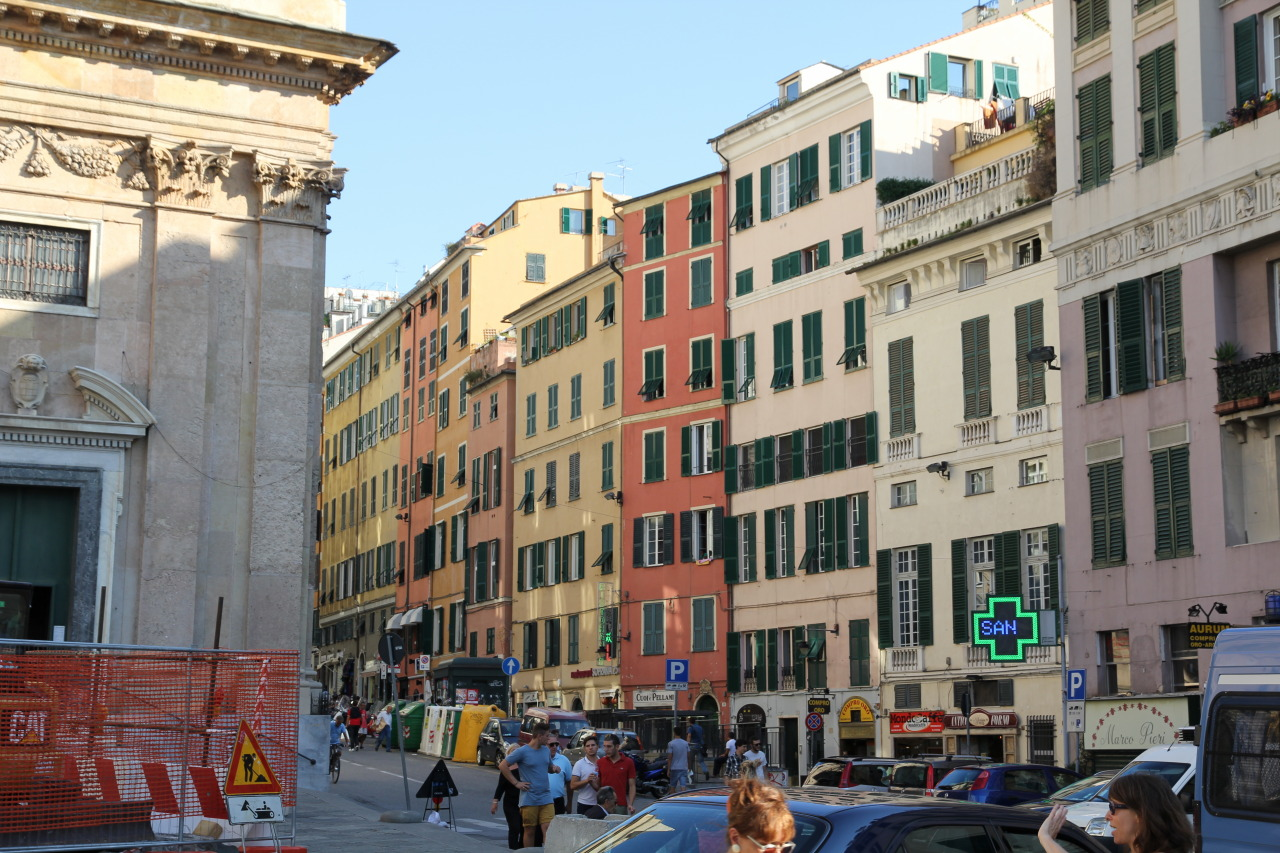
\includegraphics [width=0.3\textwidth]{../Bilder/Sardinien/3.jpg}}\quad
%   \subfloat{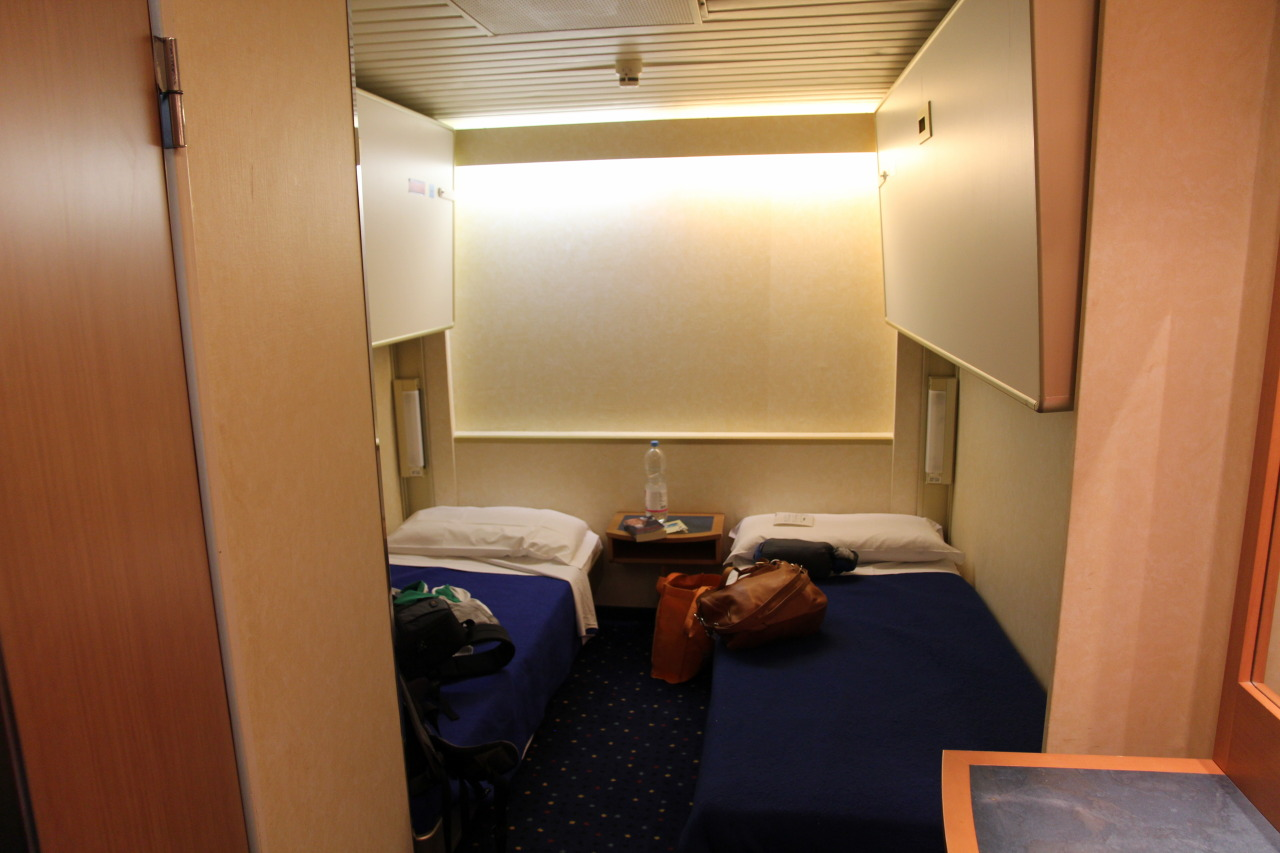
\includegraphics [width=0.3\textwidth]{../Bilder/Sardinien/4.jpg}}\quad
%   \caption[Meran]{Meran}
%\end{figure}

%\begin{figure}[hb]
%    \centering
%    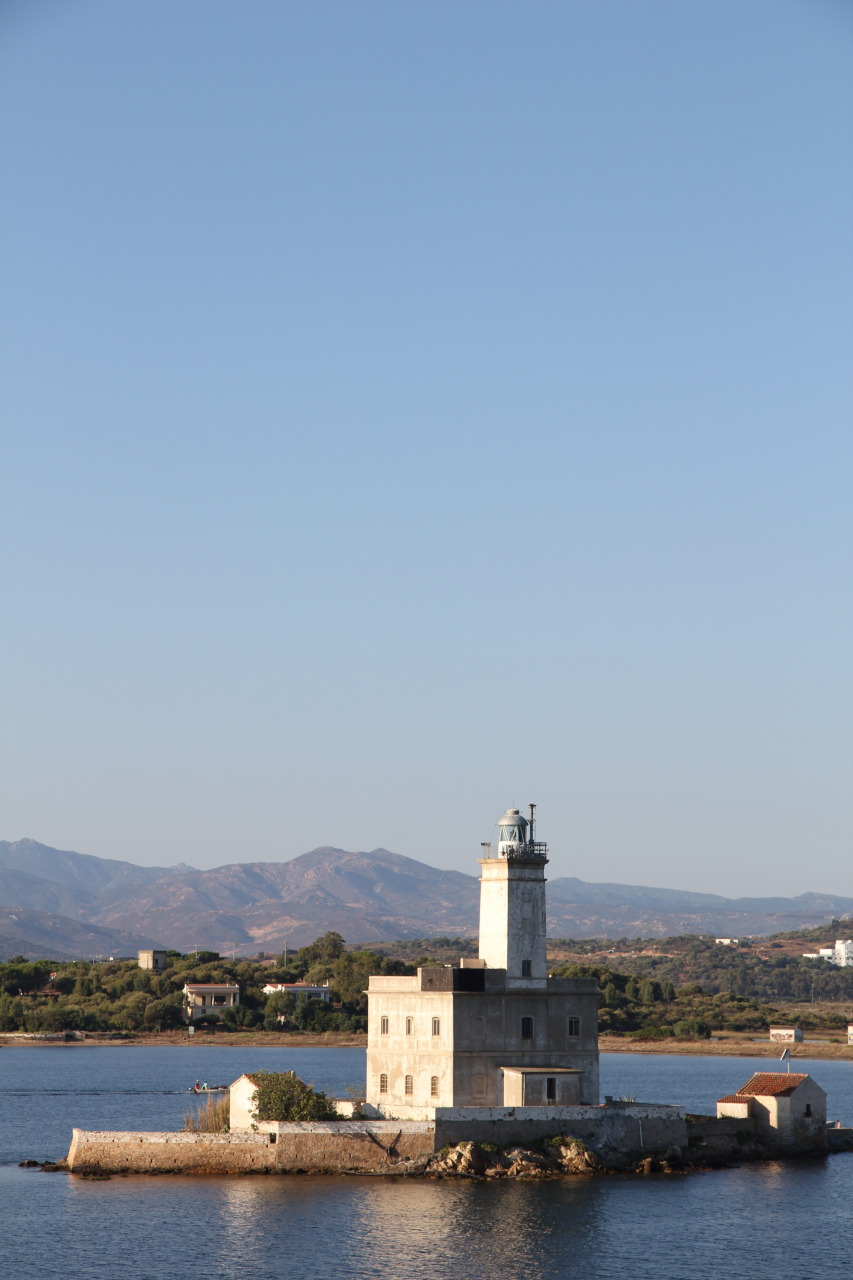
\includegraphics[width=\textwidth]{../Bilder/Sardinien/7.jpg}
%    \caption{Da sind sie ja...}
%    \label{img:Sardinien}
%\end{figure}

\subsection{Einleitung} 
Nach langem hin und her, von Bali über Thailand landeten wir am Schluss doch wieder bei den Busferien.
Der nahende Umzugstermin und damit verbundene Kosten machten die Entscheidung um einiges leichter.
Doch damit begann die Debatte um unser Reiseziel erst Elba, Sardinien, Schweden, England, ... .
Am Schluss machte Sardinien das Rennen.
Mit der Voraussetzung, dass wir nicht die ganze Insel bereisen wollten sondern schön faul einfach der Nase nach reisen wollten.
Es sollten so richtige entspannte Ferien werden.
Im nachstehenden Reisebericht kann selber nachverfolgt werden, ob uns das gelungen ist.  

\subsection{01.09.2013 Die erste Etappe} 
Da ich leider die Wäsche in  Buochs vergessen hatte war unsere erste Etappeziel Buochs.
Alles fing eigentlich schon am letzten Donnerstag an.
Nichts Böse ahnend begab ich mich in den Keller um meine Wäsche für die kommenden Ferien vorzubereiten.
Zwei volle, dröhnende Waschmaschinen hiessen mich willkommen.
Sah eher bitter aus für meine Wäsche.
Schnell Plan B zurechtgezimmert.
Am Freitag Abend alles mitnehmen und in Dättwil waschen.
Sehr schön, wenn der Herr nicht so vergesslich wäre und die Schmutzwäsche in der Zentralschweiz liegen gelassen hätte.
Ok, Plan C tritt in Aktion! Schon am Sonntagabend nach Buochs aufbrechen und noch schnell waschen.
Plan C funktionierte tadellos.
Ich liebe es wenn ein Plan funktioniert.
Vor der Abfahrt der ersten Etappe wurden wir noch mit einem feinen Nachtessen am Taubenweg verwöhnt.
Die ersten Kilometer der neuen Reise mussten so einfach gelingen.

\subsection{02.09.2013 Nichts kann uns aufhalten} 
Nach dem die Wäsche im Keller geholt war, wie auch die Gipfeli vom Beck, war es an der Zeit aufzubrechen.
Das Schiff sollte Genua zwar erst um 21:30 verlassen, doch wollten wir den Montag noch für einen kurzen Zwischenhalt in Genua nutzen.
Chantal bot sich als erste Fahrerin an, ein Umstand, welcher dankend angenommen wurde.
Schon nach kurzer Fahrt wurden jedoch Ermüdungserscheinungen sichtbar und so wurde abgemacht, dass der erste Wechsel nach dem Gotthard stattfinden sollte.
An der Raststätte Gottardo Sud wurde Jack noch einmal frisch aufgetankt und wir versorgten uns mit Pizzas und Kaffee.
Die kurze Pause und der Fahrerwechsel schienen irgendwelche schlechte Schwingungen heraufzubeschwören.
Jedenfalls fiel zuerst die Beleuchtung unserer Borduhr aus, welche erst vor wenigen Tage repariert wurde und dann machte sich auch noch die Geschwindigkeitsanzeige selbständig.
Nach einem beherzten Sprung auf 80 km/h fiel die Nadel Richtung 0 wo sie auch verweilte.
Goldig.
Nächste Ausfahrt raus und mit geschickten Handgriffen wurden die Probleme gelöst.
Es konnte weitergehen.
Die Fahrt verlief dann vollkommen ereignislos.
Auch die Parkplatz Suche in Genua verlief extremst erfolgreich.
Gleich neben dem Fähr- Terminal konnten wir einen Parkplatz ergattern und machten uns dann sogleich auf Genua zu erforschen.
Hm, Genua? Wo ist denn da das Zentrum? Wir stolperten per Zufall über eine Metro-Station.
Auf der Grafik der Linie war zu lesen, dass es einige Stationen von der aktuellen gefundenen entfernt, eine mit der Bezeichnung Zentrum zu geben scheint.
Seit wann besitzt denn Genua eine Metro? Die Erde spuckte uns wenig später bei einem eindrücklichen Brunnen wieder aus und wir machten uns auf die Suche nach etwas kalorienhaltigem.

\begin{figure}[h]
    \centering
    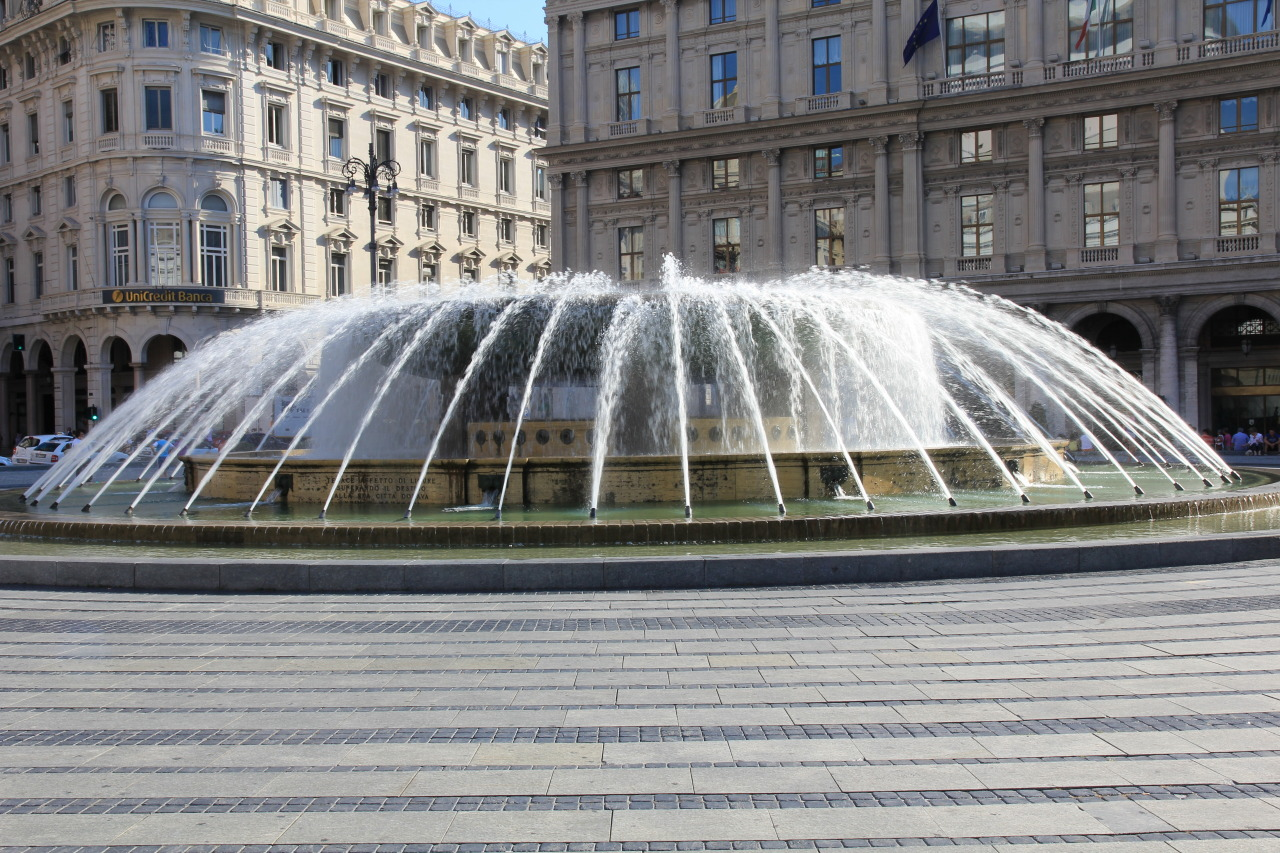
\includegraphics[width=\textwidth]{../Bilder/Sardinien/1.jpg}
    \caption{Beim diesem Brunnen wurden wir ausgespuckt}
    \label{img:Brunnen in Genua}
\end{figure}

Focaccia und der Dauerbrenner Pizza machten das Rennen.
Später wurde eine Bar aufgesucht, in der Chantal die weltgrößten Gnocchi zu sich nahm.
Die konnten es echt mit Knödel aufnehmen.
Nach einer kurzen Phase der Desorientierung fanden wir denn Weg mit dem Auto an den Check-In des Hafens.
Vielspurig wurde angestanden und begleitet durch wilde Hup-Attacken versuchten sich einzelne Ungeduldige im Anstehen.
Um etwa 20:00 Uhr waren wir auf der Fähre und konnten unser Zimmer mit Dusche beziehen.
Sofort wurde das Schiff erkundet und ein weiterer Apéro fand verdienterweise den Weg in unsere Mägen.
Kurz nach dem Ablegen ging das Licht in der Kabine 7020 aus.  

\begin{figure}[h]
   \centering
      %\subfloat[CAPTION]{BILDERCODE}\qquad
   \subfloat{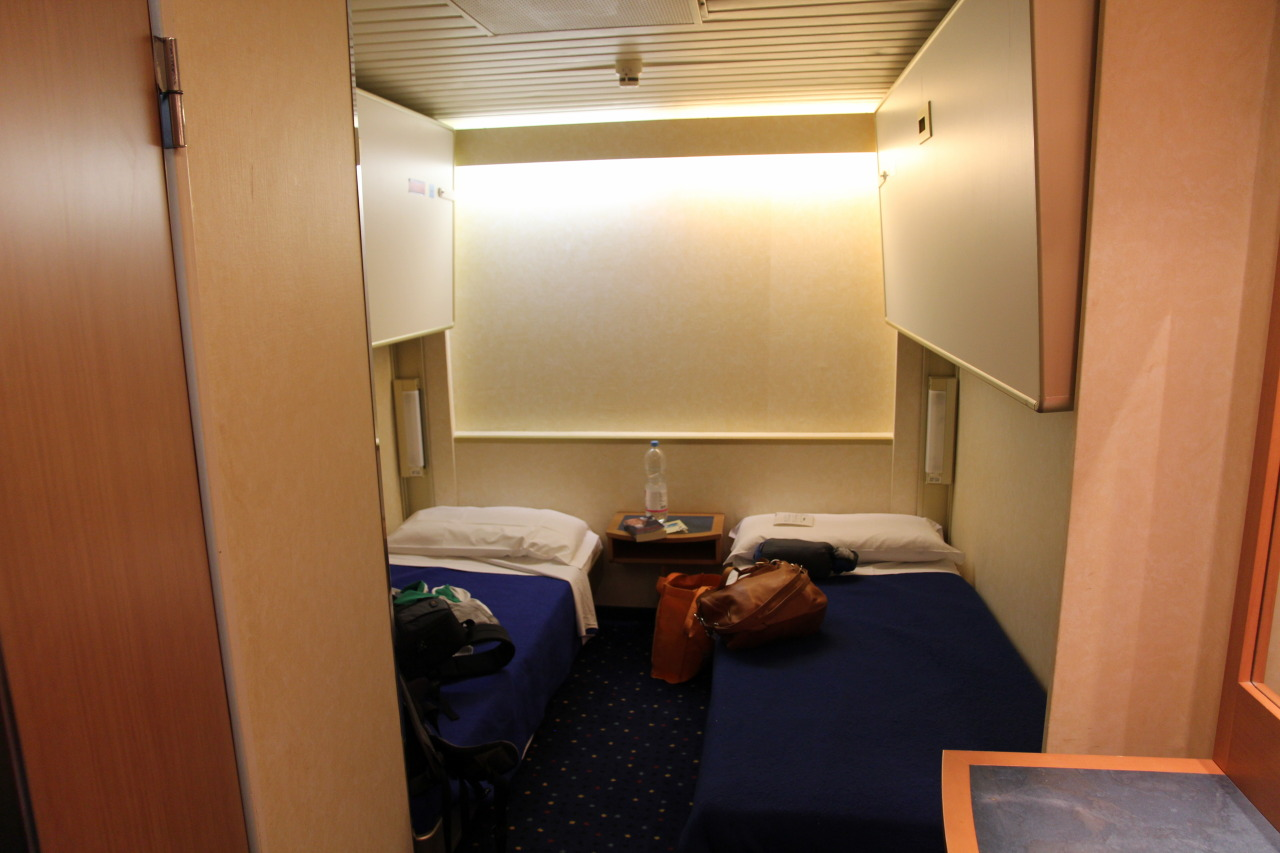
\includegraphics [width=0.3\textwidth]{../Bilder/Sardinien/4.jpg}}\quad
   \subfloat{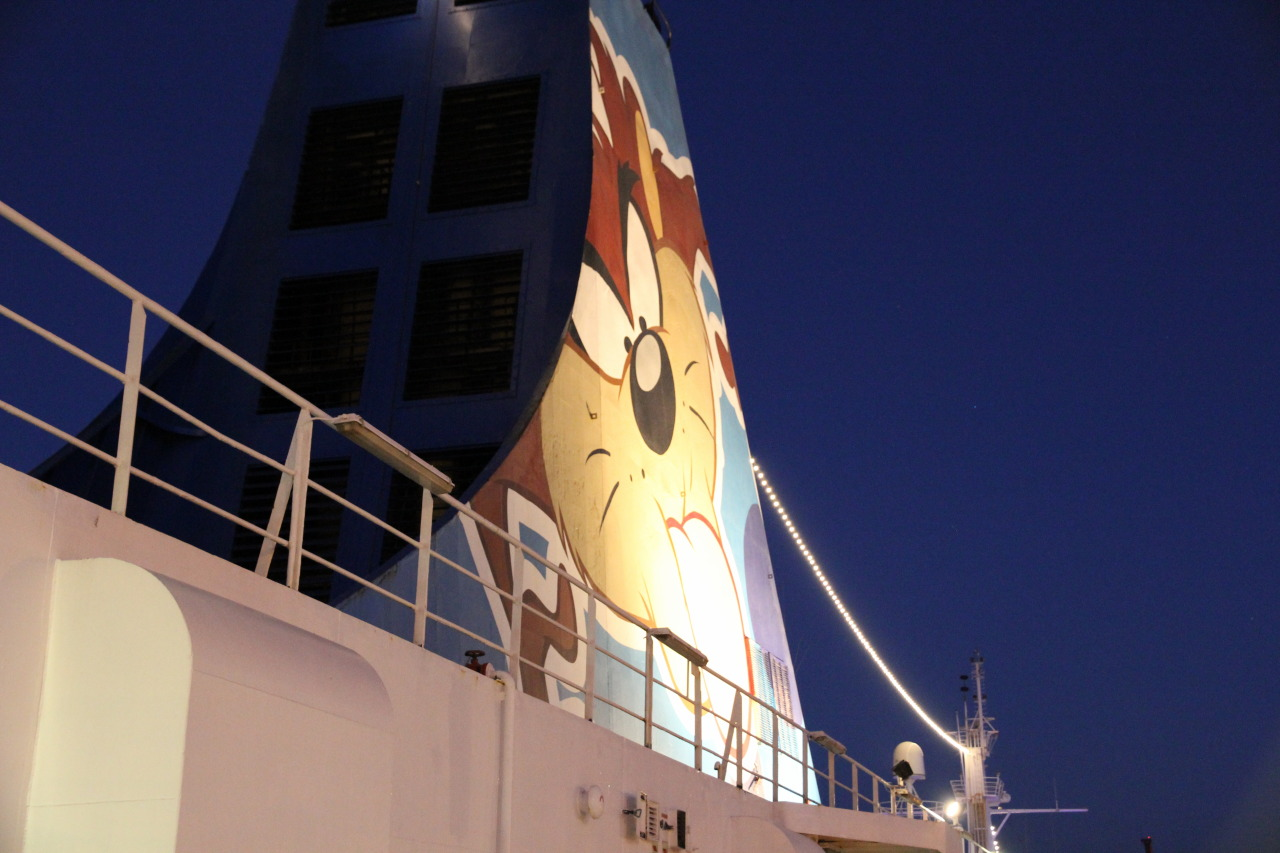
\includegraphics [width=0.3\textwidth]{../Bilder/Sardinien/5.jpg}}\quad
   \subfloat{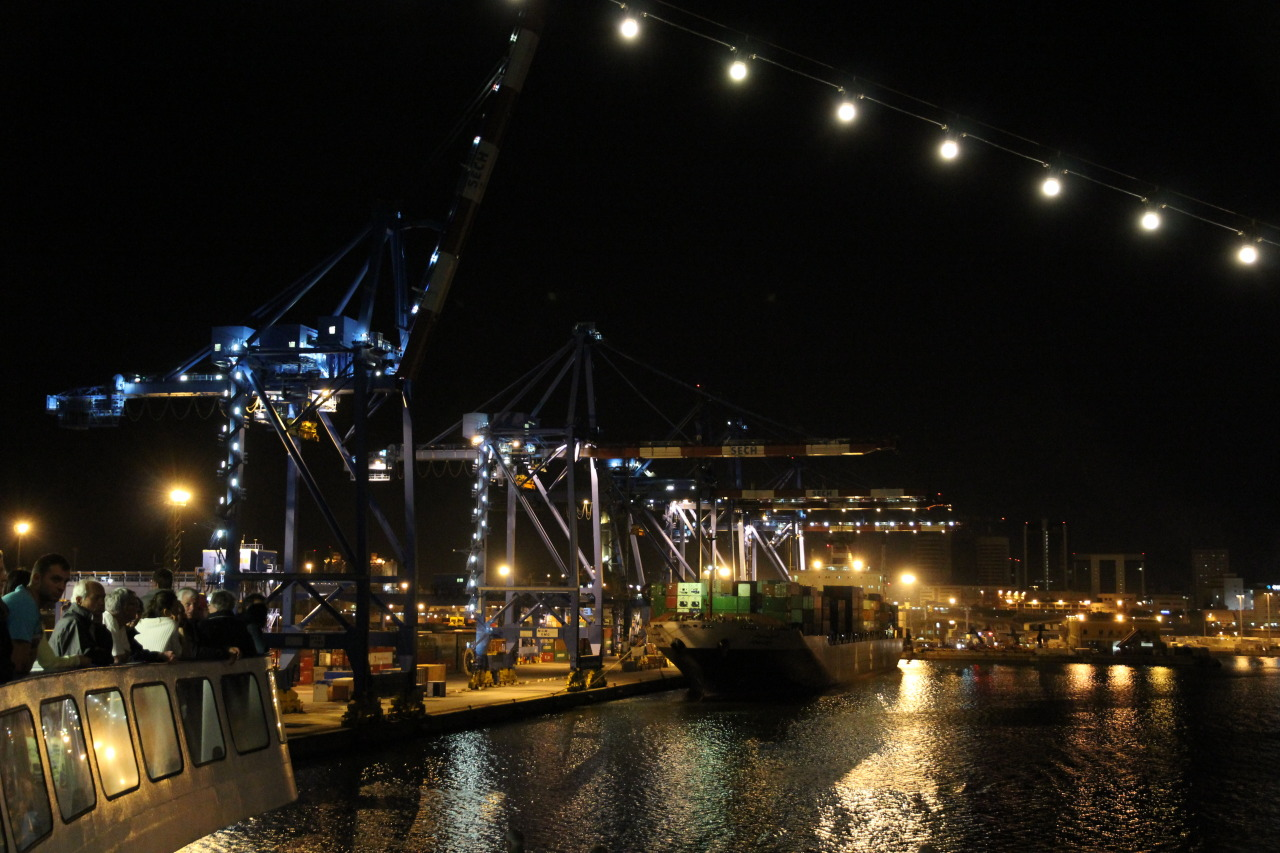
\includegraphics [width=0.3\textwidth]{../Bilder/Sardinien/6.jpg}}\quad
   \caption[Auf der Fähre]{Auf der Fähre}
\end{figure}

\newpage

\subsection{03.09.2013 Sardinien, here we are} 

\begin{wrapfigure}{L}{0.3\textwidth} 
  \begin{centering}
    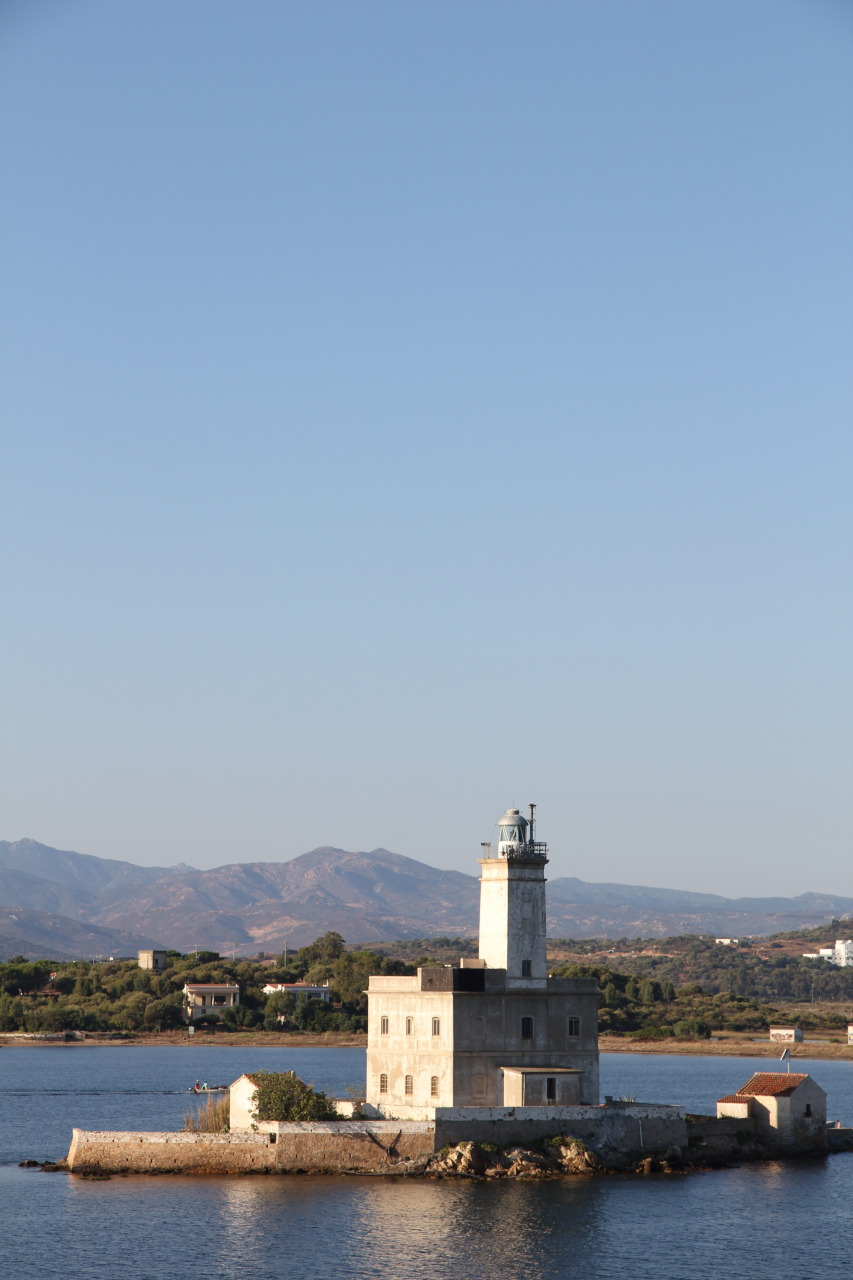
\includegraphics[width=0.4\textwidth, height=5cm, keepaspectratio]{../Bilder/Sardinien/7.jpg}
    \caption{Einfahrt in den Hafen}
  \end{centering}
\end{wrapfigure} 

Erst der Wecker konnte mich aus dem Schlaf reisen, welcher durch das leichte Schaukeln des Schiffes noch tiefer als normal ausfiel.
Chantal meinte jedoch das sie eher schlecht geschlafen hätte und sich wunderte, dass ich nicht durch ihre nächtliche Ranggerei aus dem Schlaf gerissen wurde.
Schnell geduscht und dann einmal einen Blick auf die Landschaft riskiert.
Per Lautsprecher wurden schon wilde Italienische Durchsagen überbracht, die das Ziel ankündigten.
Noch kurz auf Deck 6 das Restaurant besucht und schon bremste das Schiff ab, um die letzten Kilometer gemächlich durch die enger werdende Hafeneinfahrt zu fahren.
Möwen boten sich für eine weitere Fotosession an und schnell wurden ein paar Bilder zu viel auf den Chip gebannt.
Wir beschlossen zuerst die Costa Smeralda zu besuchen und steuerten direkt ein viel gelobter Strand an.
Wie schon im Reiseführer beschrieben führte eine eher holprige Piste die letzten 2 km bis zum Parkplatz, welcher von einem jungen Herr bewacht wurde.
Kurz ein Zettel bei dem Typen abgeholt und schon konnte der kurze Spaziergang zum Strand beginnen.
Das Wasser war unglaublich klar und der Sand bot zum verweilen ein, was wir auch taten.
Ein Blick auf die Uhr überraschte uns.
Erst 10 Uhr.

\begin{figure}[b]
   \centering
      %\subfloat[CAPTION]{BILDERCODE}\qquad
   \subfloat{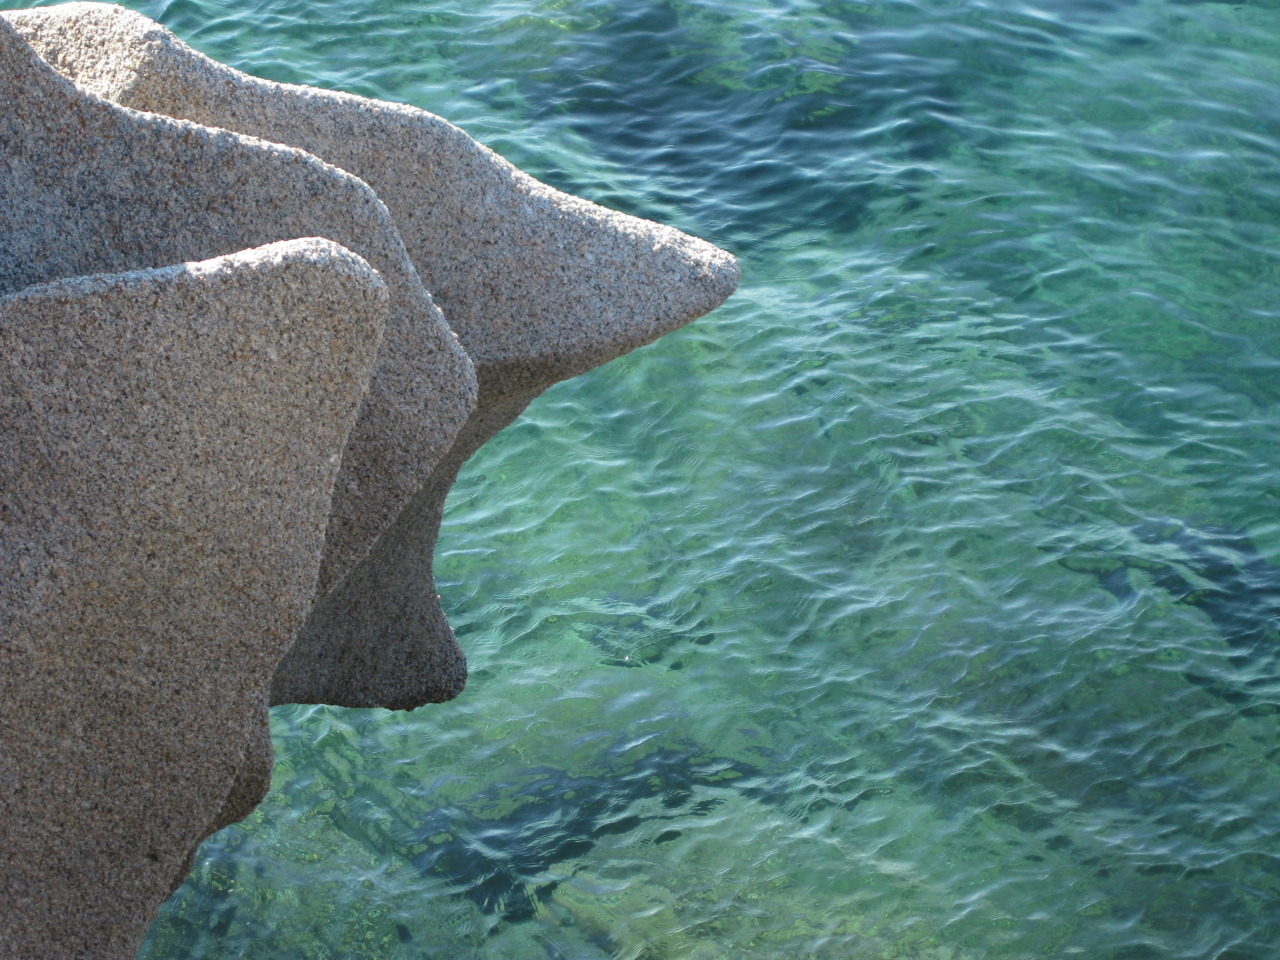
\includegraphics [width=0.3\textwidth]{../Bilder/Sardinien/13.jpg}}\quad
   \subfloat{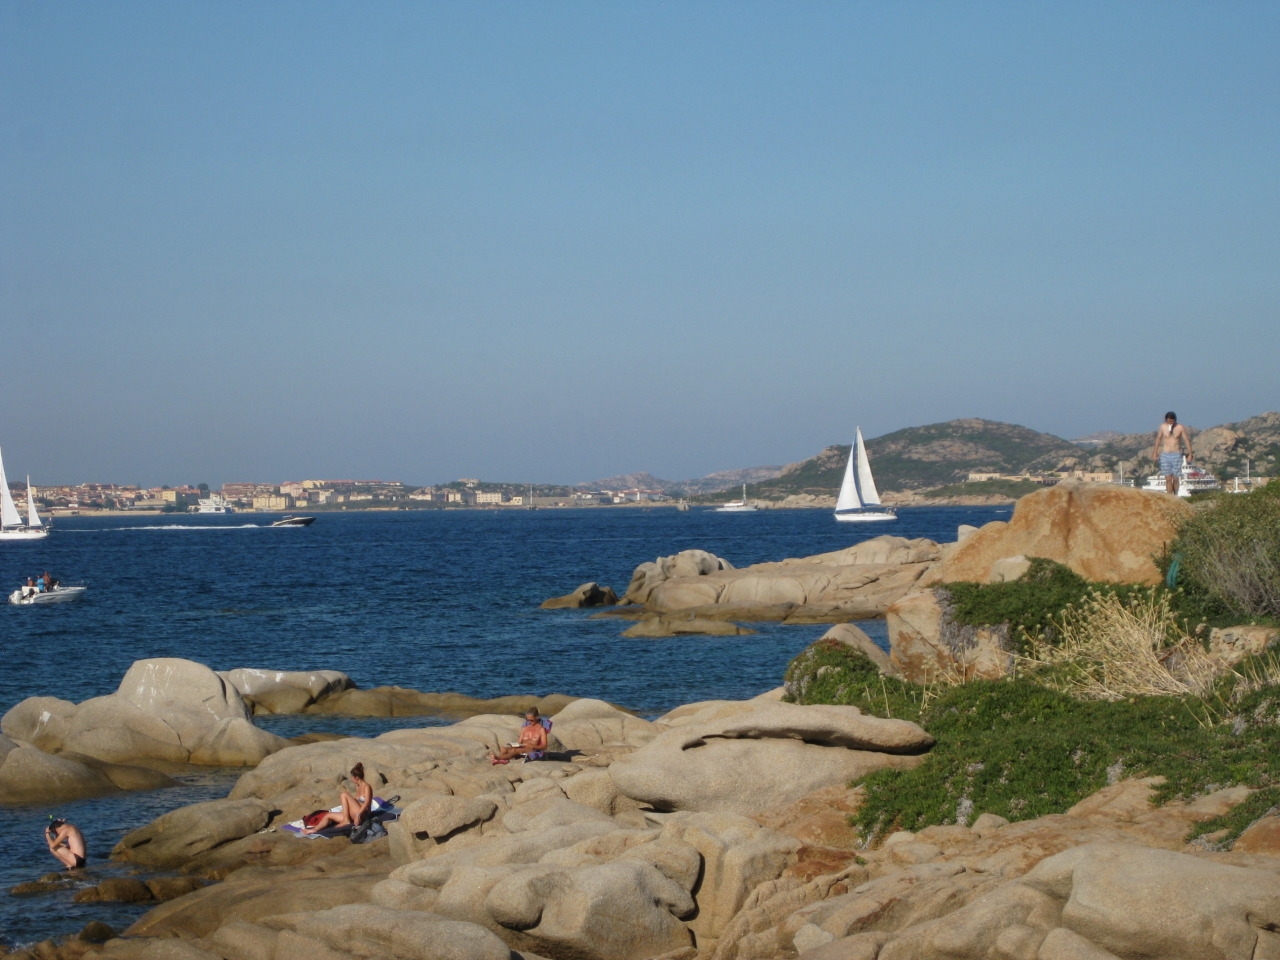
\includegraphics [width=0.3\textwidth]{../Bilder/Sardinien/14.jpg}}\quad
   \subfloat{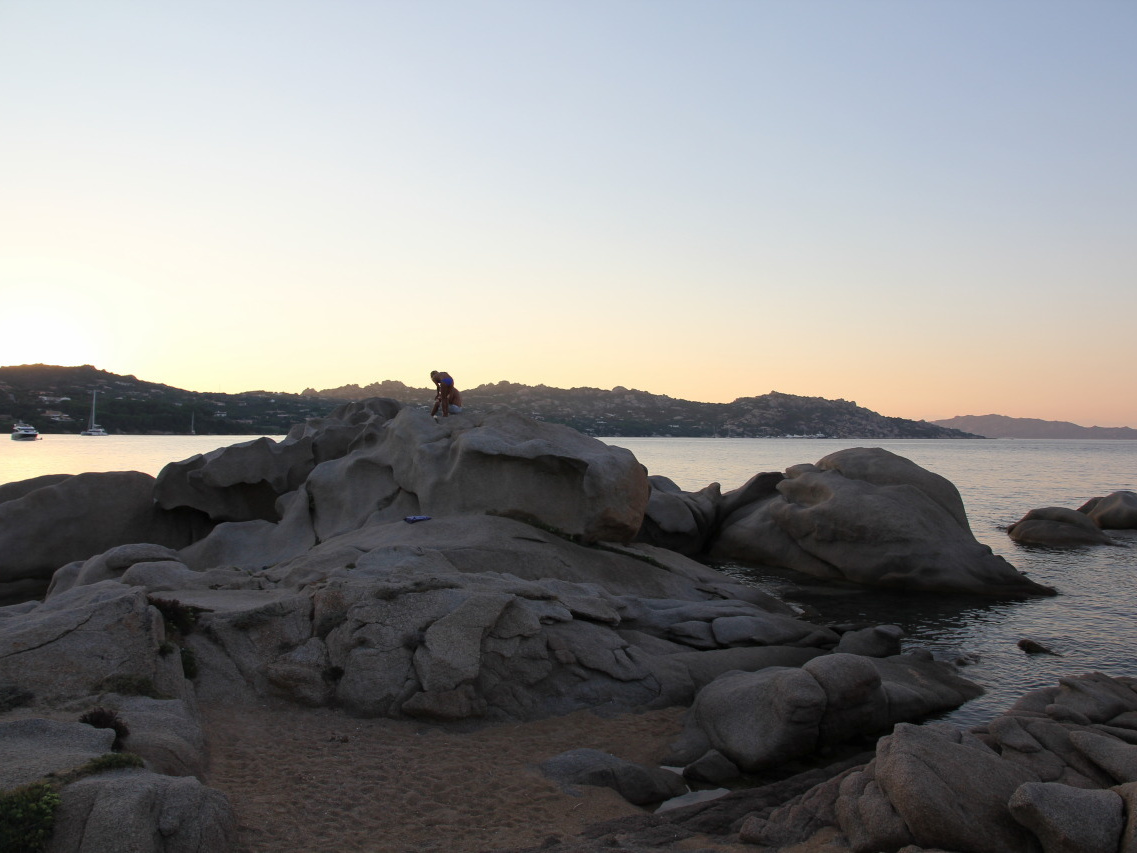
\includegraphics [width=0.3\textwidth]{../Bilder/Sardinien/15.jpg}}\quad
   \caption[Unser erster Campingplatz]{Unser erster Campingplatz}
\end{figure}

Dank der erlernten Sonnenschirmeingrabtechnik deluxe vom letzten Sommer war auch das anbringen desjenigen problemlos.
Am Nachmittag folgte ein kurzer Besuch der Bar am Strand und gegen 16:00 kündigten die ersten roten Streifen am Körper die Notwendigkeit den Platz an der Sonne zu räumen an.
Unser erstes Nachtlager sollte in der Nähe von Palau aufgeschlagen werden.
Auch dieser Weg wurde dank den überirdischen Helferlein problemlos gefunden.
Der interessant gelegene Campingplatz war leider jedoch ziemlich voll, so dass nur noch ein eigentlicher Abstellplatz für uns übrig blieb.
Es wurde jedoch Besserung für den nächsten Tag in Aussicht gestellt.
Der Platz eigene Strand war wunderschön und Chantal machte sich sofort an die Analyse der verschiedenen Gesteinsarten.
Wir wollten dann Richtung Palau radeln, jedoch stoppte ein platter Reifen an einem der Fahrräder das Vorhaben schon im Ansatz.
Glücklicherweise habe ich für diese Reise so ziemlich alles an Werkzeug mitgenommen, was mir über den Weg gelaufen ist und so war auch diese Panne relativ schnell behoben.
Das kleine Dörfchen Palau hatten wir schnell erkundet und auch ein Gefühl in der Magengegend kündigte ein nötiges Abendessen an.
Ein Geschäft für Sonnenbrillen lockte uns dann trotzdem noch über die Türschwelle und sogleich wurde ich fündig.
Das ausgesuchte Restaurant war ein Volltreffer.
Nach Melonen mit feinem Schinken waren Spaghetti al Cozze und Sardinische Gnocchi (Pasta mit Tomatensauce und scharfen Würstchen; normale Gnocchi sind viel besser) auf dem Tisch und zu guter Letzt noch eine Goldbrasse.
Zurück beim Camping war die Erleichterung über das vollständig zum Pfus-Bus umgemöbelte Fahrzeug schier greifbar.

\subsection{04.09.2013 Warten auf die Ösis} 
Nach einer schönen langen Nacht erwachten wir erst gegen 10:00 Uhr und einer der ersten Blicken galt dem uns versprochenen Stellplatz direkt am Meer.
Leider war dort immer noch ein weisser VW-Bus darauf geparkt.
Nach einem kurzen Frühstück, bei dem uns natürlich das Gas im Gaskocher ausging, war der Stellplatz immer noch besetzt.
Chantal machte sich zur Rezeption auf um Klarheit zu schaffen.
Die frohe Botschaft war, dass der Deutsche den Platz noch heute räumen soll.
Kurz darauf wurde das Gespräch mit dem Stellplatzbesetzer aufgesucht, mit dem Ergebnis, dass er eigentlich im Sinne habe noch länger zu bleiben.
Konfusion.
Der Nachbar jedoch wolle heute noch abreisen.

\begin{figure}[hb]
    \centering
    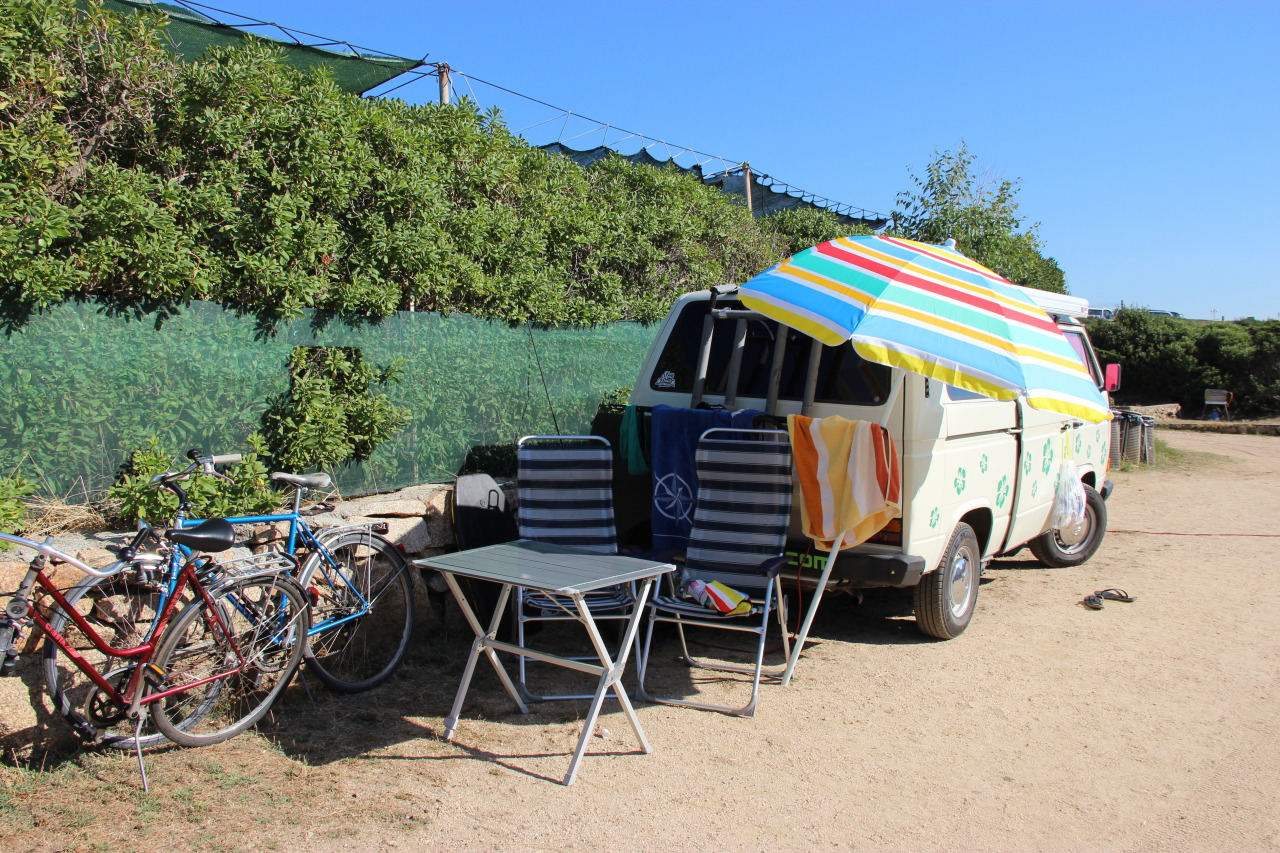
\includegraphics[width=\textwidth]{../Bilder/Sardinien/17.jpg}
    \caption{Unser eher provisorischer Stellplatz}
    \label{img:Sardinien1}
\end{figure}

Aha, ab jetzt wird also der Österreicher beäugt und bei der kleinsten Bewegung des Gefährts wird unser Startklar gemacht und auf den neu eroberten Stellplatz verschoben.
Wir verbrachten den Tag mit baden in allen Varianten.
Endlich kam auch mein Bodyboard zum Einsatz.
Mit Schnorchel und Brille bewaffnet statteten wir der Unterwasserwelt einen Besuch ab.
Doch auch  immer wenn wir auftauchten der unliebsame Platzbesetzer war noch auf \glqq unserem\grqq{} Platz.
Gegen 17:00 machten wir uns todesmutig trotz der immer noch bemerkenswerten Hitze auf den Weg nach Palau um die Lebensmittelvorräte aufzustocken.
Als wir zurückkamen waren die Ösis doch tatsächlich immer noch da.
Nach dem Genuss des Sonnenunterganges bildete sich eine wahre Menschentraube um den schon öfters erwähnten Stellplatz.
Es wurde wild diskutiert, wer jetzt denn diesen Platz besetzen möchte.
Der italienische Platzwart setzt dem Rummel ein Ende und erklärte den herumstehenden was Sache ist.
Nach dem umstellen von Jack genossen wir die Sicht auf das Meer aus Reihe eins.
Zur Feier des Platzes kochten wir Orechiette und versuchten uns in der Dämmerungsfotografie.
Danach war schon bald die Energie aufgebraucht und wir legten uns zum sanften Plätschern der Wellen hin.

\begin{figure}[H]
   \centering
      %\subfloat[CAPTION]{BILDERCODE}\qquad
   \subfloat{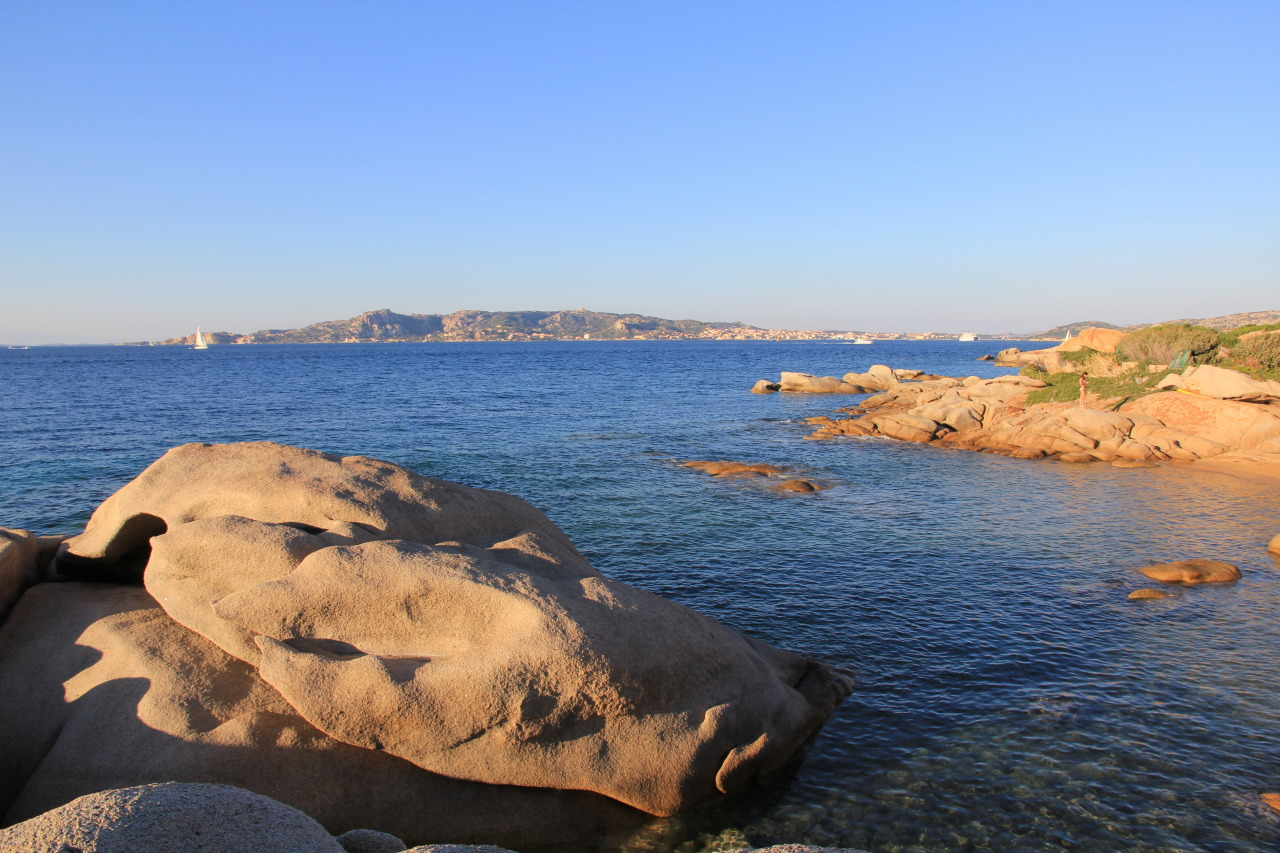
\includegraphics [width=0.3\textwidth]{../Bilder/Sardinien/20.jpg}}\quad
   \subfloat{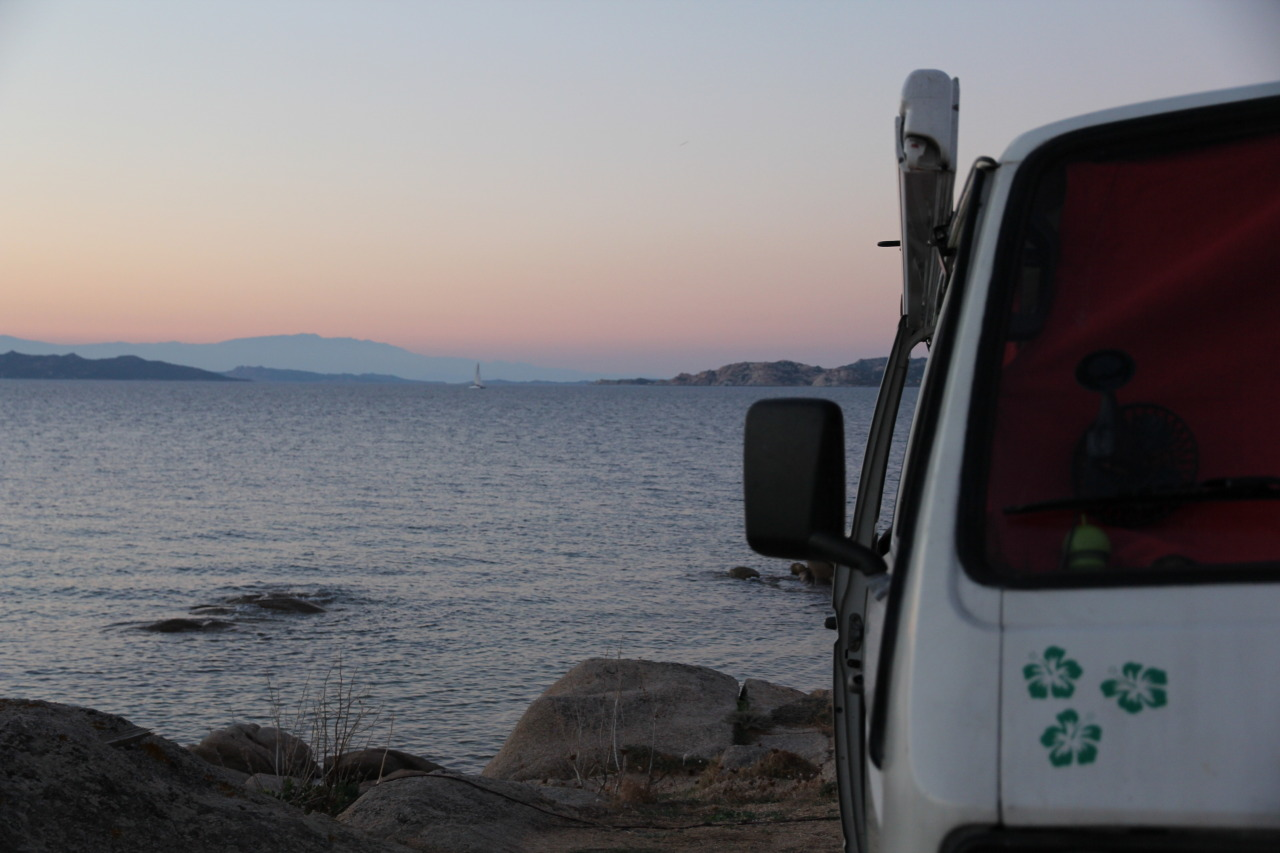
\includegraphics [width=0.3\textwidth]{../Bilder/Sardinien/22.jpg}}\quad
   \subfloat{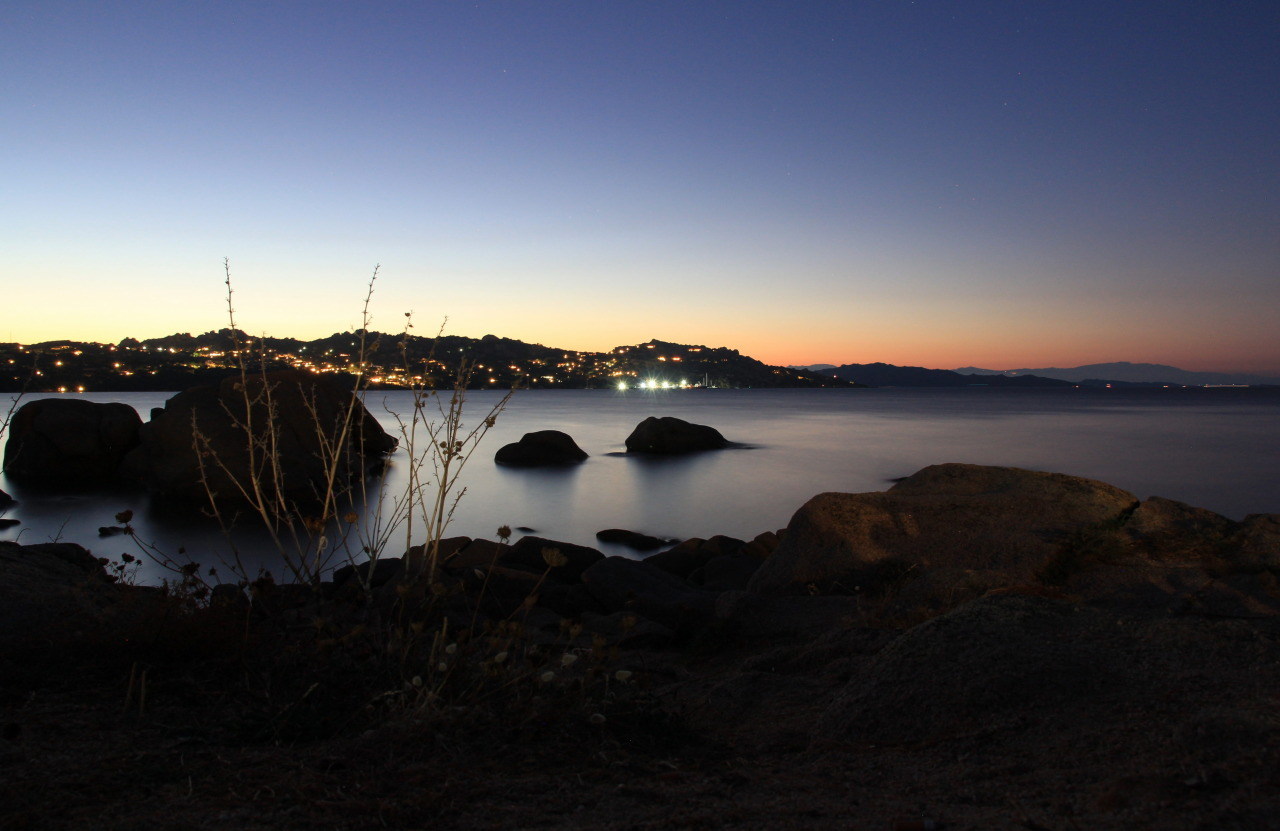
\includegraphics [width=0.3\textwidth]{../Bilder/Sardinien/24.jpg}}\quad
   \caption[Impressionen vom Mee]{Impressionen vom Meer}
\end{figure}

\begin{figure}[hb]
    \centering
    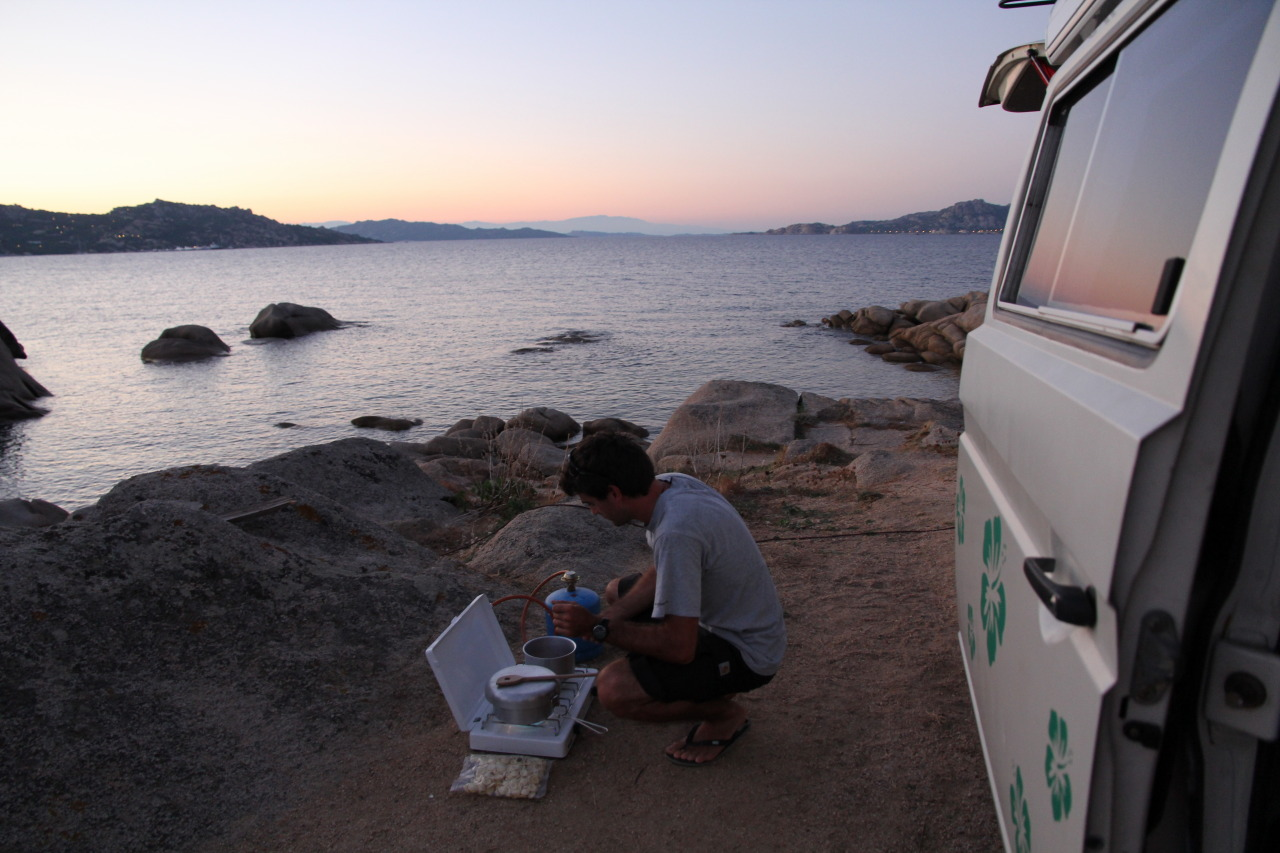
\includegraphics[width=0.95\textwidth]{../Bilder/Sardinien/23.jpg}
    \caption{Wunderschöner Platz, leider nur für eine Nacht}
    \label{img:Sardinien2}
\end{figure}

\newpage

\subsection{05.09.2013 Boaah eyyy} 

\begin{wrapfigure}{L}{0.3\textwidth} 
  \begin{centering}
    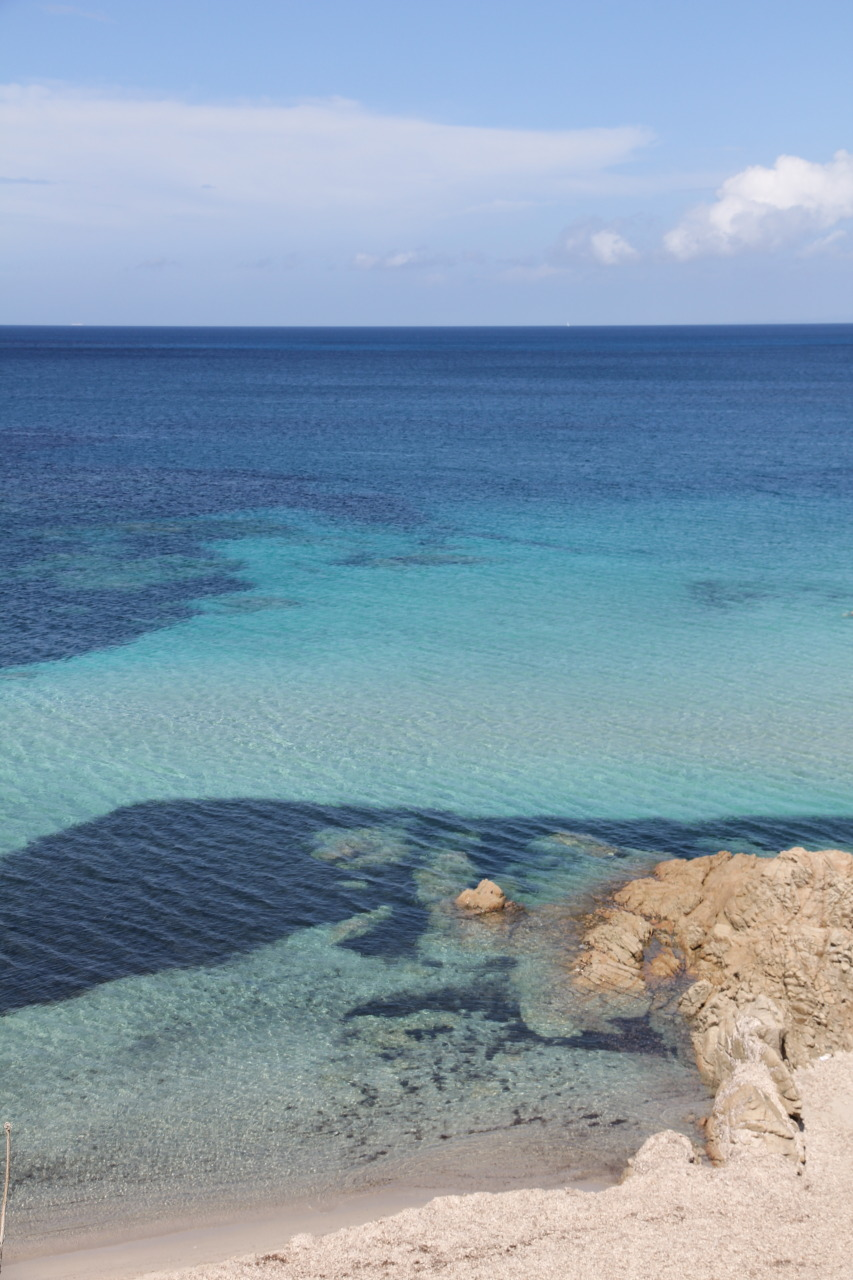
\includegraphics[width=0.4\textwidth, height=6cm, keepaspectratio]{../Bilder/Sardinien/27.jpg}
    \caption{Traumhafter Strand}
  \end{centering}
\end{wrapfigure} 

Ein weniger schönes Plätschern und Grollen begrüsste uns zum heutigen Tag.
Es goss wie aus Kübeln.
Ohne Rücksicht auf Verluste stürzte ich mich aus dem Bus um unsere Badetücher vor dem drohenden ertrinken zu retten.
Danach ging es noch einmal zurück in den trockenen Teil des Busses.
Genau auf das Frühstück getimt kam jedoch die Sonne hinter den Gewitterwolken hervor und trocknete alles wieder auf ein erträgliches Mass ab.
So war es nach der ersten Verpflegung des Tages auch kein Problem, alles in den Bus zu räumen und uns für einen neuen Platz umzusehen.
Bevor wir jedoch den Platz verlassen konnten, standen schon alle mögliche Gegenstände von den sich aufdrängenden Nachbesitzer auf dem Platz.
Wie die Geier fielen sie über den frei werdenden Platz.
Jack lief wunderbar und die etwa 2 Stündige Fahrt Richtung Valledoria konnte beginnen.
Die Landschaft war eher trocken, jedoch von wunderbaren Sträuchern reich mit Blumen behangen unterbrochen.
Aus dem Augenwinkel sahen wir kurz ein wunderbar türkis leuchtender Strand aufblinken und schon wurde der Blinker gestellt um diese potentielle Schönheit zu betrachten.
Tatsächlich, der Strand war nahezu perfekt.
Unglaubliches Bild!  Zuerst war der Plan nur kurz runter zuschauen, doch schon bald waren wir uns einig auch die Flossen ins Wasser zu halten.
Herrlich!! Nur der Wind machte unserem Sonnenschirm arg zu schaffen und auch das aufkommende Unwetter konnte uns dann irgendwann davon überzeugen dieses wunderbare Fleckchen Erde zu verlassen. 

\begin{figure}[hb]
    \centering
    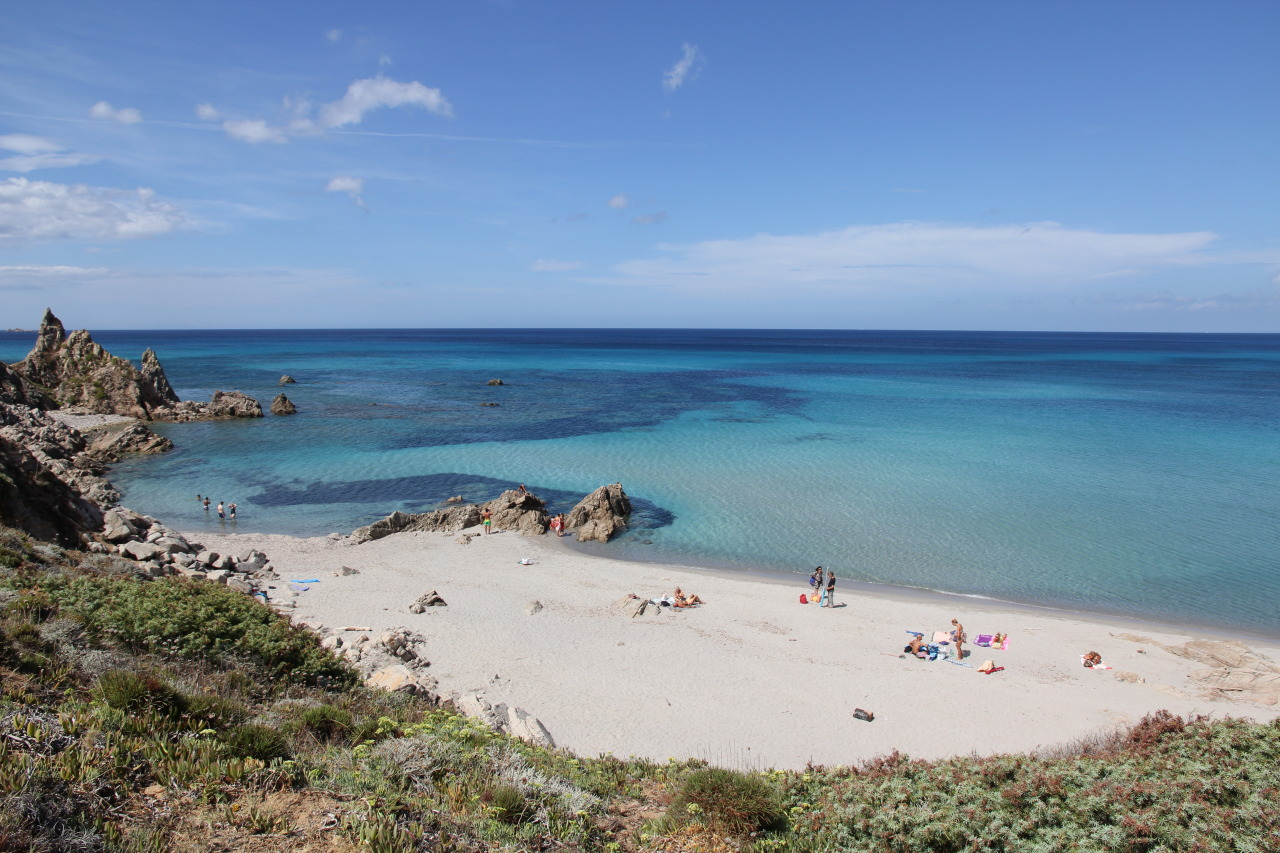
\includegraphics[width=0.95\textwidth]{../Bilder/Sardinien/26.jpg}
    \caption{Wunderschöner Platz, leider nur für eine Nacht}
    \label{img:Sardinien3}
\end{figure}

\begin{figure}[H]
   \centering
      %\subfloat[CAPTION]{BILDERCODE}\qquad
   \subfloat{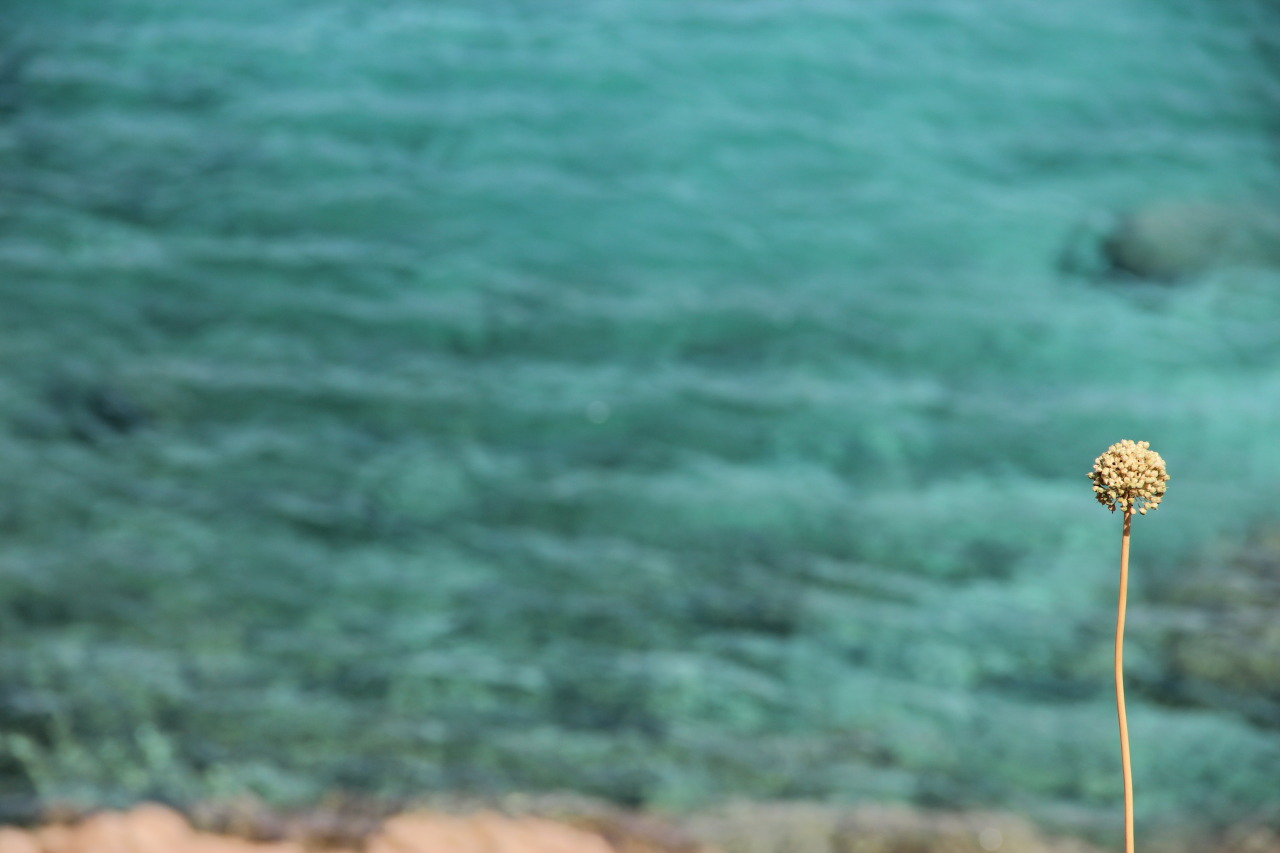
\includegraphics [width=0.3\textwidth]{../Bilder/Sardinien/30.jpg}}\quad
   \subfloat{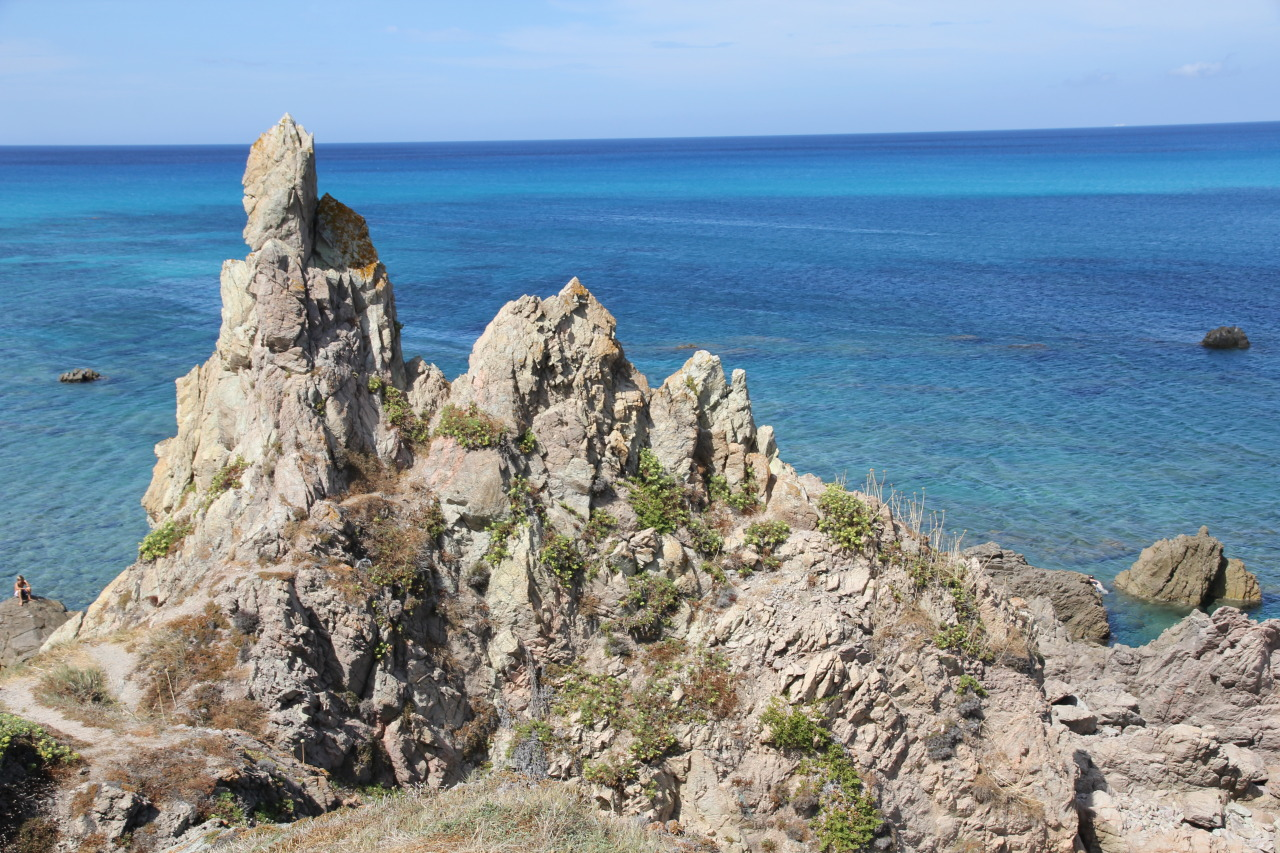
\includegraphics [width=0.3\textwidth]{../Bilder/Sardinien/28.jpg}}\quad
   \subfloat{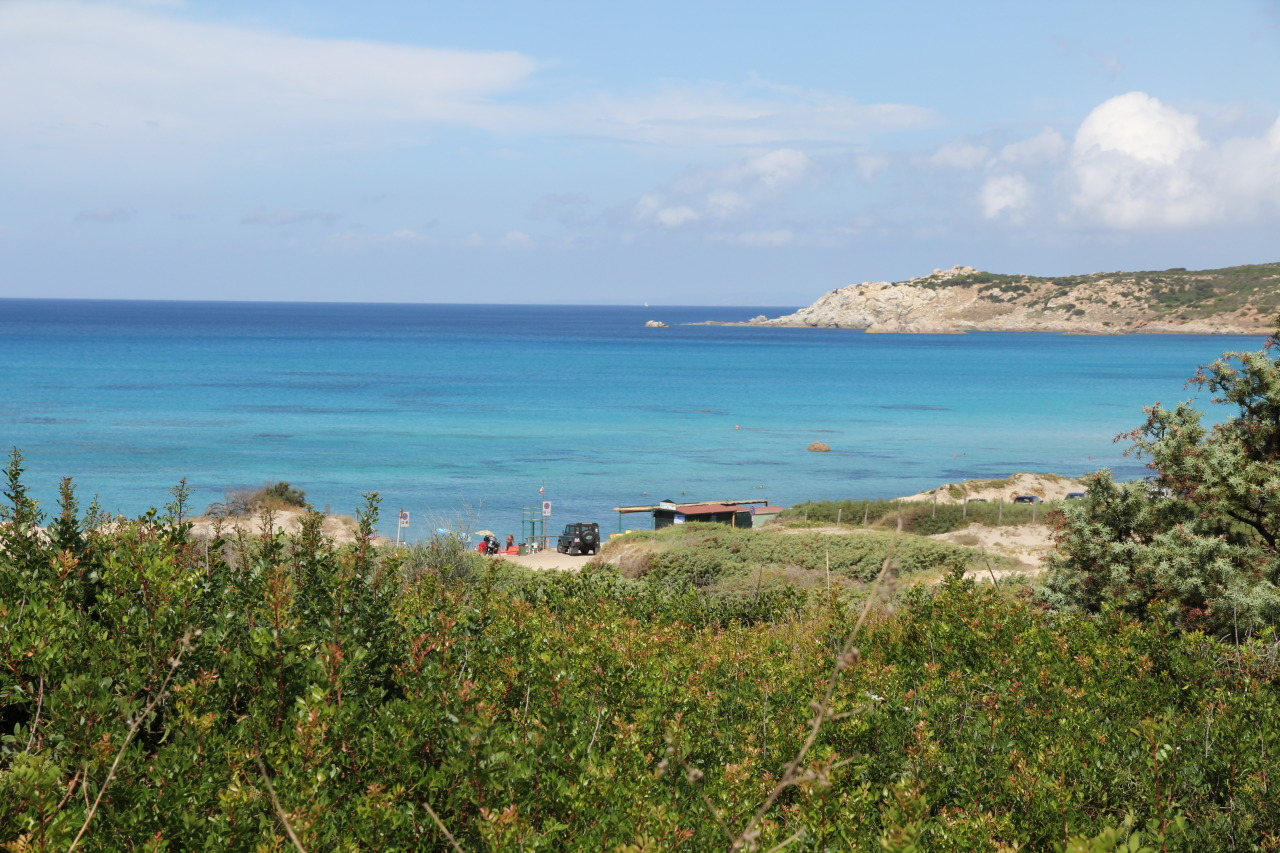
\includegraphics [width=0.3\textwidth]{../Bilder/Sardinien/25.jpg}}\quad
   \caption[Impressionen vom Mee]{Impressionen vom Meer}
\end{figure}

Auf den Überlandstraßen kamen wir sehr gut vorwärts und wir näherten uns schon bald Valledoria.
Zwischenzeitlich noch kurz den Weinvorrat aufgestockt und schon waren wir auf dem riesigen Campingplatz la foce.
Nachdem wir in Rekordzeit den Platz bezogen hatten, ging es Richtung Städtchen.
Naja, Strasse würde es eher beschreiben.
Trotzdem war es uns möglich die letzten Punkte der Einkaufsliste abzuarbeiten.
Ein nicht gerade einladendes Restaurant, das aber sehr gut besucht war, zog unsere Aufmerksamkeit auf sich.
Die Lautstärke in dem Lokal war ohrenbetäubend.
Etliches Bedienpersonal flitzte zwischen den Tischen hindurch und 2 Pizzaiolo warfen nur so mit Mafiatorten um sich.
Trotz geschätzten 90 Gästen die alle bedient werden wollten, wurde die Bestellung in Rekordzeit geliefert.
Während wir mit der immens großen Pizza die Mägen füllten, wollten auch noch unzählige Einheimische eine Pizza über die Gasse beziehen.
Der Pizzaofen glich  dem Baregg zu seinen besten Zeiten.
In Reihe verließen die übergroßen Scheiben den Ofen.
Der süffige Wein tat sein bestes und auch so konnten wir einen weiteren schönen Tag auf Sardinien beschließen.  

\subsection{06.09.2013 Tendenz nach links} 
Der Vorsatz früher aufzustehen und damit der größten Hitze des Tages zuvorzukommen wurde schon im Keim erstickt.
Unser sportliches Ziel von heute war nichts geringeres als die Eroberung des Fjordes per Kajak.
Nach einem ausgiebigen Frühstück, welches uns bestens auf das Abenteuer vorbereitete, schmierten wir uns mit mehreren Lagen Sonnencreme ein und setzten unser Entdecker Gesicht frei nach Kolumbus auf.
Schon bei den ersten Paddelschlägen mit unserem gemieteten Kajak mussten wir leider einen leichten Links Drall feststellen.

\begin{figure}[H]
   \centering
      %\subfloat[CAPTION]{BILDERCODE}\qquad
   \subfloat{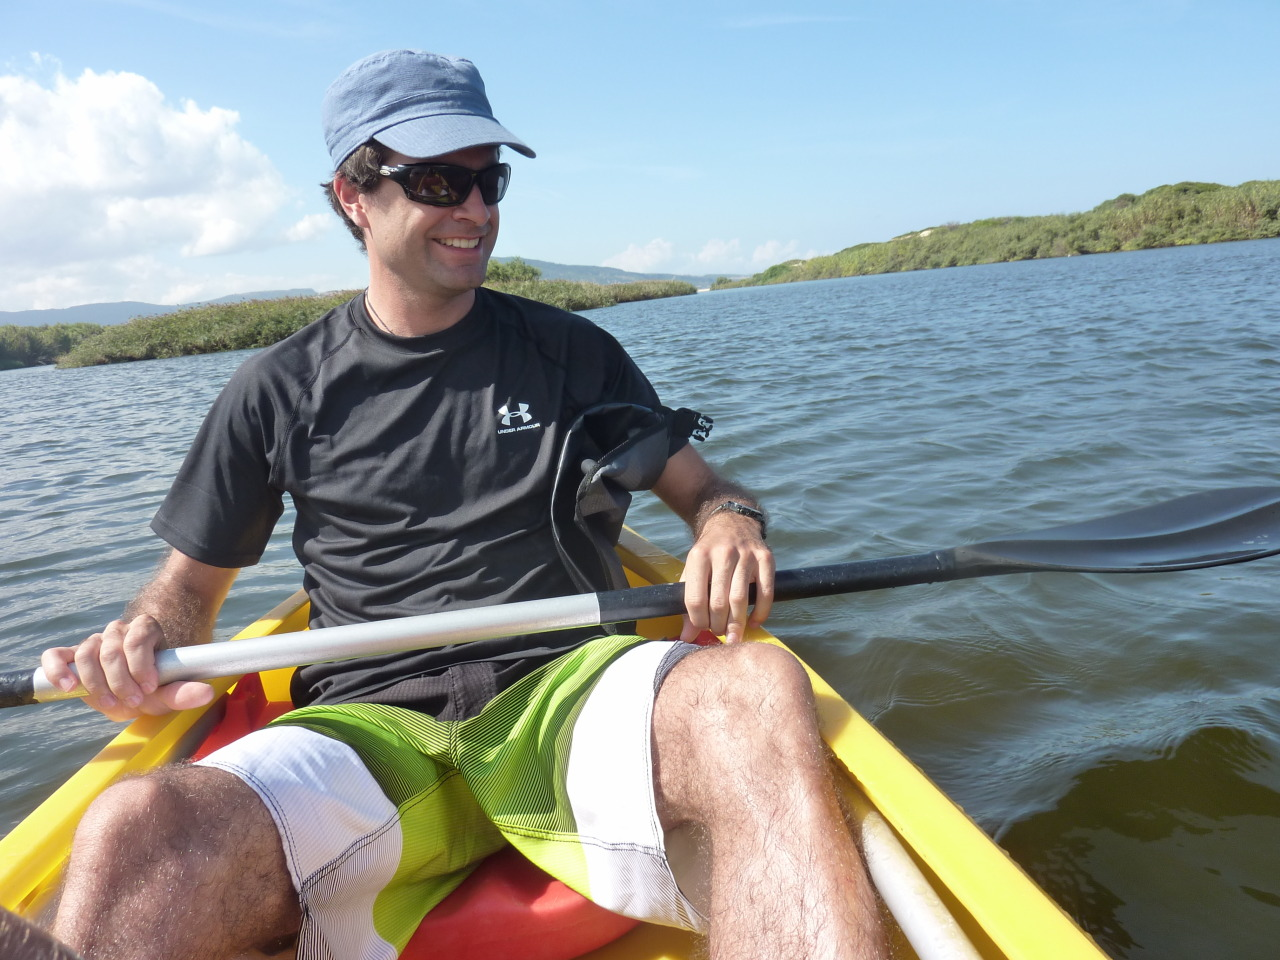
\includegraphics [width=0.3\textwidth]{../Bilder/Sardinien/34.jpg}}\quad
   \subfloat{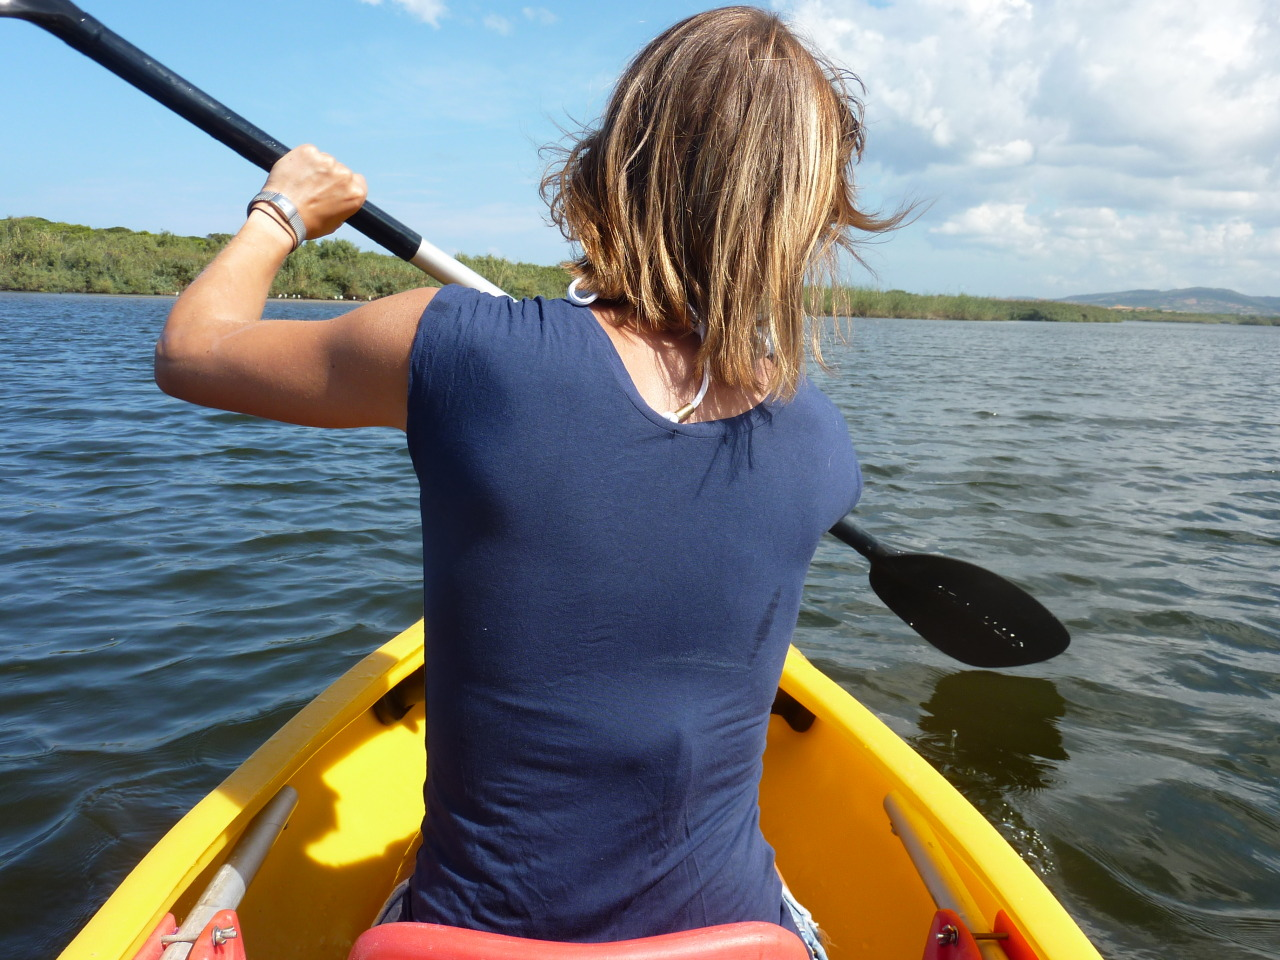
\includegraphics [width=0.3\textwidth]{../Bilder/Sardinien/33.jpg}}\quad
   \subfloat{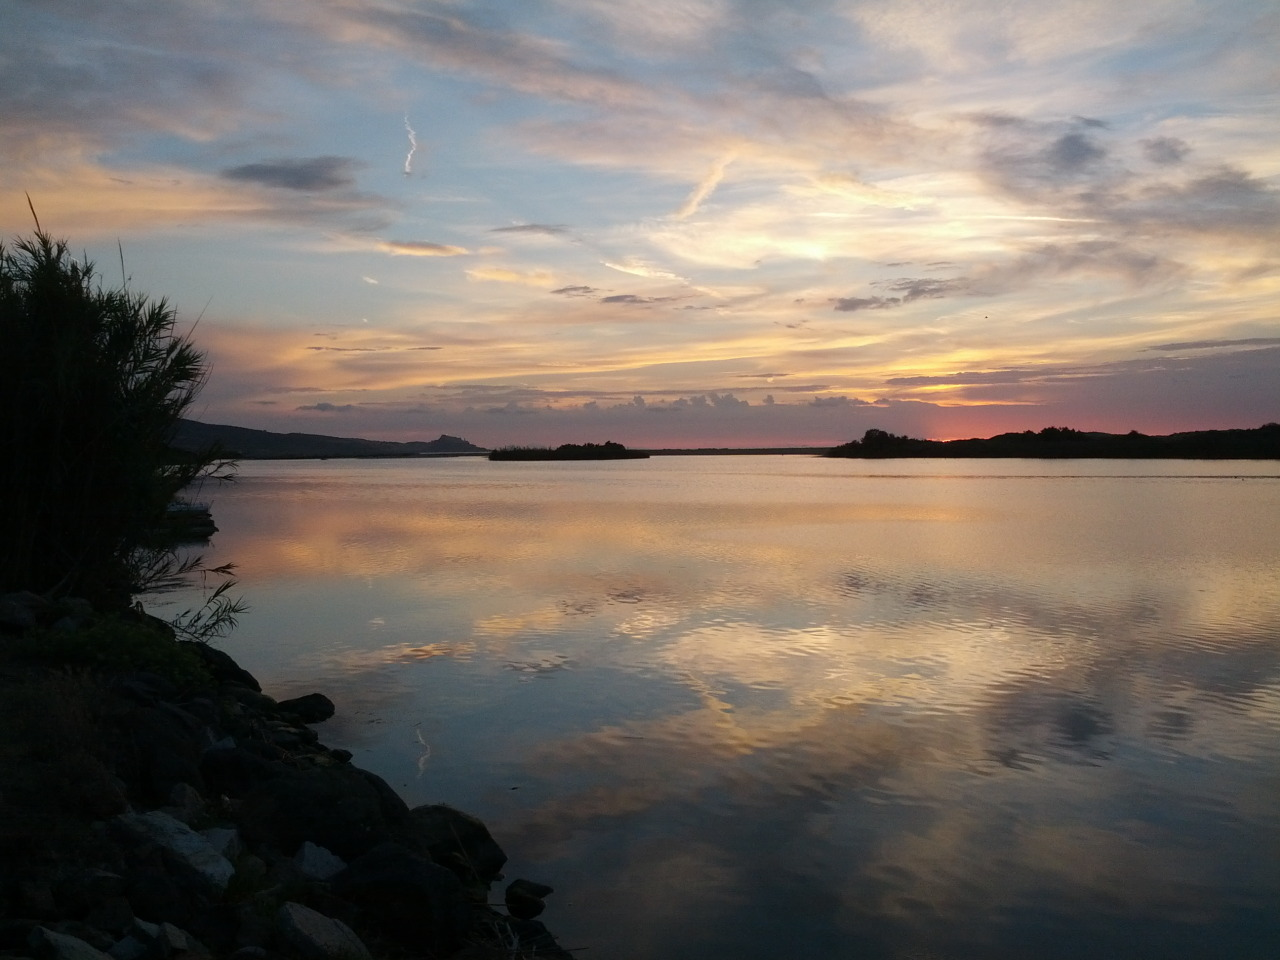
\includegraphics [width=0.3\textwidth]{../Bilder/Sardinien/32.jpg}}\quad
   \caption[Kajak]{Kajak}
\end{figure}

Die gegen uns arbeitende Strömung tat ihr Bestes uns an unserem Vorhaben zu behindern.
Die anfängliche Motivation sank auf der vorderen Ruderstation schneller als auf der hinteren.
Trotz allem, paddelten wir gut eine Stunde gegen die Strömung und wurden mit fliegenden Fischen und Eisvögeln für die Schinderei belohnt.
Richtung Vermietstation ließ es sich dann doch eher leichter und schneller paddeln und nach gut 1.
5 Stunden hatte uns das Festland wieder und unsere Erkundungstour by boat nahm ein Ende.
Gegenüber dem Fjord befand sich  mehrere Kilometer lange Sandstrand welche wir mit etwas Sonnenbaden beehren wollten.
Der Camping eigene Fährdienst, der die Überquerung des Fjordes möglich machen sollte, befand sich gerade in der Siesta.
Nach kurzer Wartezeit war er auf seinem Boot und der 3 Minuten Trip konnte beginnen.
Auf der anderen Seite der Düne hieß uns ein starker Wind willkommen, der uns jedoch gerade recht war.
Dadurch war das verweilen am Strand sehr angenehm und die drohenden roten Nasen schlichen sich unbemerkt an.
Die nachmittägliche sportliche Betätigung im Kajak bewirkte nicht gerade eine Steigerung im Können beim Beachball.
Ausrede gefunden und sowieso das sehr günstige wenn nicht billige Spielequipment schmeichelte unserem Potential jetzt auch nicht gerade.
Kurz vor 17:00 Uhr beschlossen wir wieder zum anderen Ufer überzusetzen und unseren reichlichen Apero-Vorräte anzuzapfen, eine Dusche zu genießen und weitere Pläne für unsere Reise zu schmieden.
Das Essen wurde dann ganz faul im Camping eigenen Restaurant zu sich genommen.
Nach einem kurzen Besuch der Bar war die Matratze viel zu verlockend und wir fielen Müde ins Bett.

\begin{figure}[hb]
    \centering
    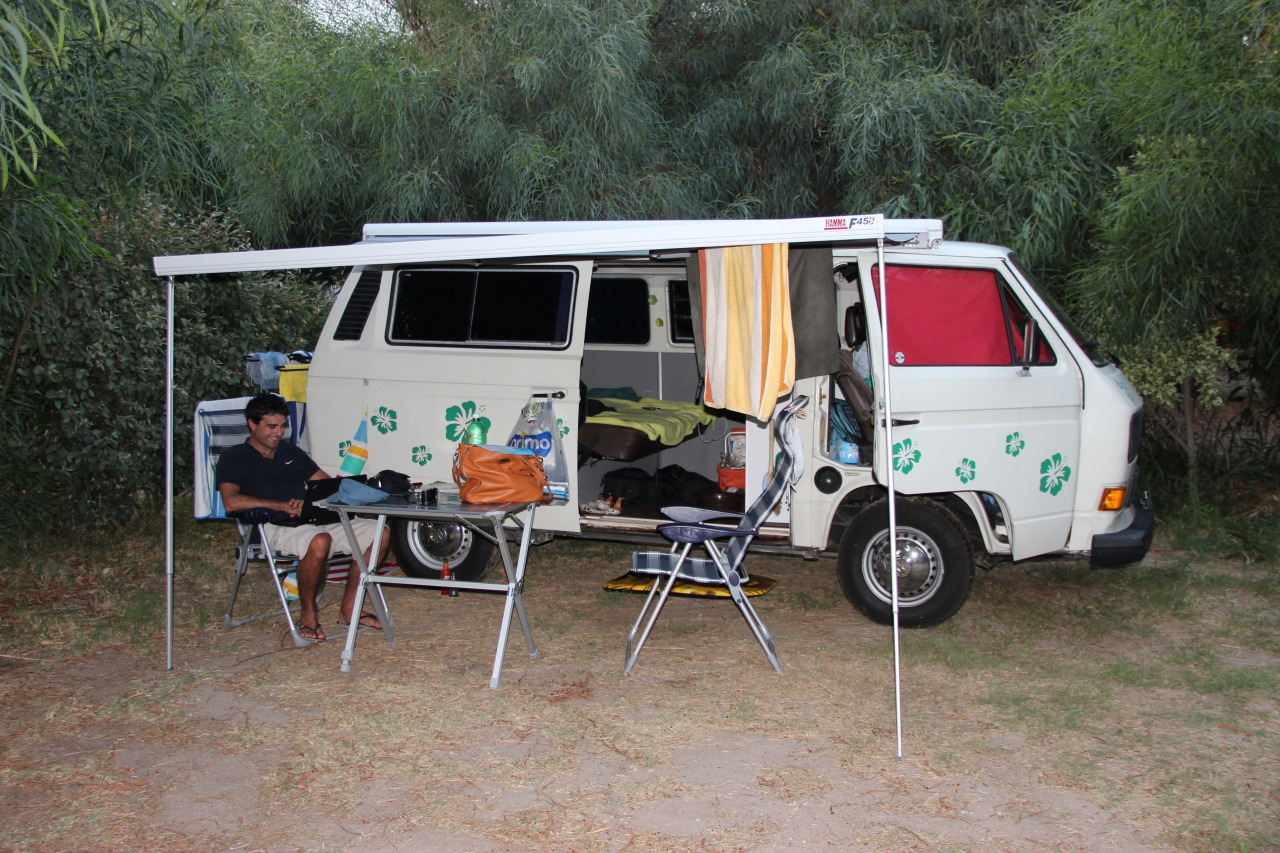
\includegraphics[width=0.95\textwidth]{../Bilder/Sardinien/38.jpg}
    \caption{Jack in seinem Element}
    \label{img:Sardinien4}
\end{figure}

\newpage

\subsection{07.09.2013 Na wohin gehts denn da?} 

\begin{wrapfigure}{L}{0.4\textwidth} 
  \begin{centering}
    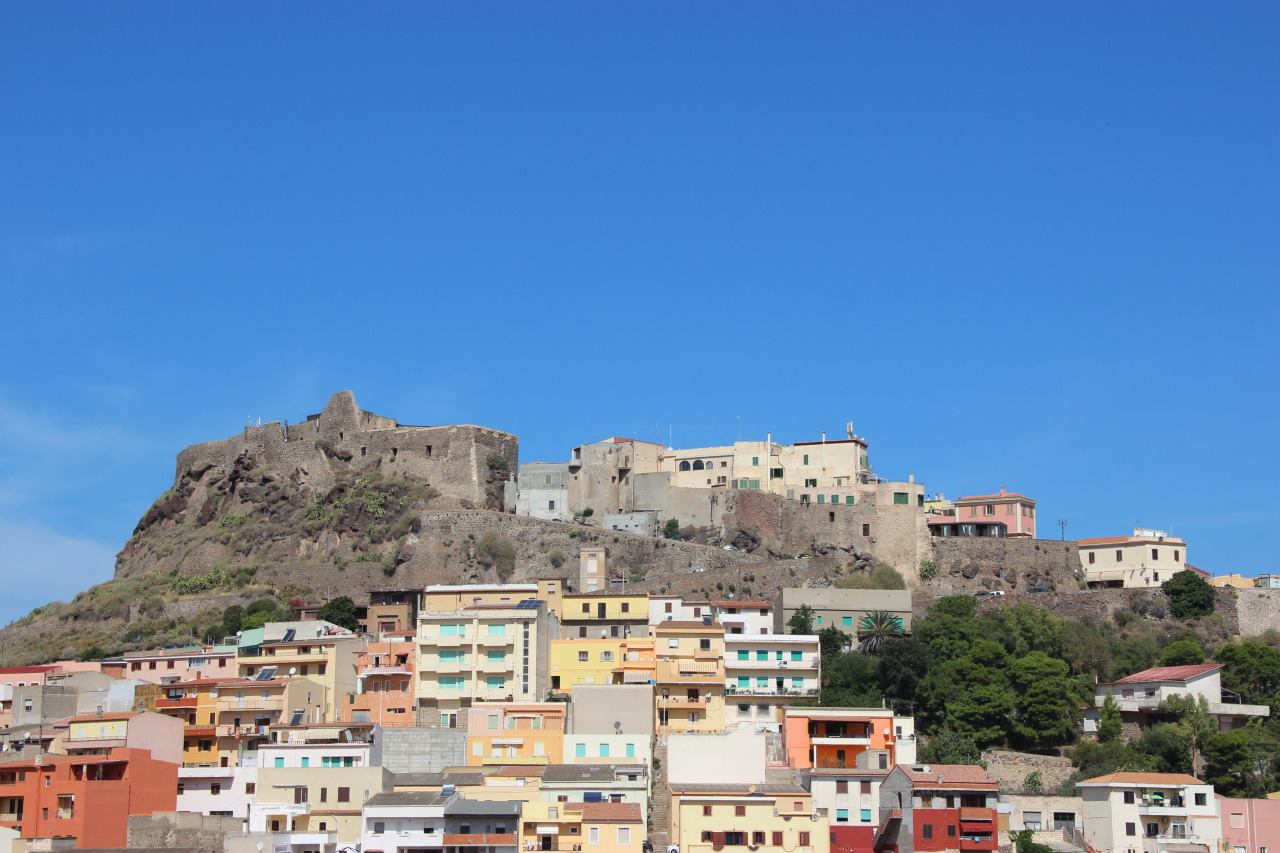
\includegraphics[width=0.4\textwidth, height=6cm, keepaspectratio]{../Bilder/Sardinien/40.jpg}
    \caption{Castelsardo}
  \end{centering}
\end{wrapfigure} 

Erst kurz vor 10:00 erwachten wir und eigentlich sollte es heute ja ein gutes Stück vorwärts gehen.
Etappenziel war Alghero mit einem Zwischenhalt in Castelsardo.
Das Packen verlief problemlos und auch der Campingplatz war überraschend preiswert.
Als wir zum Bezahlen neben der Rezeption parkten, stiess Jacks Halbbruder dazu.
Auch ein weisser VW-Bus aus dem Aargau, jedoch nicht mit Blumen sondern mit Kamelen geschmückt.
Nach einem kurzen Gespräch mit den Besitzer des Busses machten wir uns auf den Weg zu unserem Zwischenziel, welches wir schnell erreichten.
Der grosse Parkplatz rief Erinnerungen an unser negativ Ereignis vor einem Jahr hervor.
Trotzdem wurde das schmucke Städtchen erkundet und einige Fotos fanden den Weg auf unsere Speicherkarte.
Noch ein von Hand geflochtener Korb für die neue Wohnung käuflich erworben und schon machten wir uns auf den Rückweg zum Auto.
Chantal entsorge kurzerhand ihre Gelatti im Abfall und als wir das Auto erreichten lief der Schweis schon in Strömen.
Kein Lüftchen zerteilte die beträchtliche Hitze.
Eigentlich seltsam, da die Lage der Stadt etwas anderes vermuten liess.
Von drei Seiten mit Wasser umgeben nahmen wir an auf eine frische Brise zu treffen.
Falsch gedacht.
Kurz nach dem wir auf dem wir uns auf den Weg nach Alghero gemacht hatten, lotste uns das Navi völlig in den Käse.
Die Schnellstraße auf der wir sehr gut vorwärtskamen, wurde durch Quartierstrassen ersetzt.
Nach 5 Minuten war der Spuk vorbei und wir waren wieder auf einem Weg, der diesen Namen auch verdient.
Der angesteuerte Zeltplatz liegt etwa 5 Kilometer ausserhalb von Alghero.
Eine Distanz die wir dank dem Velo problemlos meistern können.
Als Begrüßung ging bei Jack zuerst einmal die Alarmanlage ab.
Der Platz ist immens.
Nach dem Auspacken des allernötigsten, hiess es zuerst einmal dösen.
Nach der Dusche sattelten wir die Velos und machten uns auf nach Alghero.
Eine wirklich schöne Stadt, welche von einer Stadtmauer umgeben ist, die begangen werden kann.
Der Apéro war super und wir nutzen den Sonnenuntergang für einige Fotos.
Das Nachtessen konnte dann niemand aus den Socken hauen.
Nach der Verpflegung schlenderten wir durch das Städtchen und meine bessere Hälfte machte sogleich einen Markt aus.
Die 5 Kilometer radeln wurden durch einen kurzen Besuch in einer Bar unterbrochen und schon bald darauf ging der Kampf gegen die drohende Mückenplage los.
Irgendwann wird es Zeit Jack ganz in ein Mückennetz zu verpacken. Gute Nacht!

\subsection{08.09.2013 An neue Ufer} 
Heute war es an der Zeit eine größere Strecke zurückzulegen.
Wir wollten die Küste wechseln um auch ein Stück der Ostküste zu begutachten.
Nach einem ausgiebigen Frühstück hiess es ein weiteres Mal packen und wir machten uns auf gen Osten.
Chantal fuhr die erste Teilstrecke der insgesamt etwa 3,5 Stunden dauernden Fahrt.
Gerade die Strecke die Chantal übernahm war sehr kurvig.
Zuerst musste sie sich aus Alghero raus kämpfen und nachher begleiteten uns kurvige enge Strassen- Nach dem Fahrerwechsel bogen wir auf eine fast Autobahn ähnliche Schnellstrasse ein und die nächste Zeit verbrachen wir in absolut unbewohnten Gebiet, welches nur durch einzelne grössere Dörfer unterbrochen wurde.
Auffälligerweise war die Strasse in einem sehr guten Zustand solange wir uns im Niemandsland bewegten.
Durch die Dörfer war eher eine Aneinanderreihung von Schlaglöcher denn eine Strasse zu sehen.
Als wir gut eine halbe Stunde von unserem Ziel entfernt waren, erhob sich unser letztes Hindernis vor uns.
Eine Bergkette, welche den Zugang zum Meer versperrte.
Eine wirklich mickrige Strasse führte über einen Pass und die fast senkrechte, dem Meer zugewandte Seite wieder runter.
Leider wurde die spektakuläre Sicht ein wenig durch den bedeckte Himmel abgewertet.
Unten im Dörfchen angekommen fanden wir den angestrebten Zeltplatz schnell.
Schon beim einchecken waren auffällig viele Schweizer zu sehen.
Unter Pinienbäume und in unmittelbarer Nachbarschaft von anderen VW-Bussen fanden wir einen schönen Platz und stellten routiniert unsere sieben Sachen auf.
Beim ersten Besuch des Dorfes am Abend stellten wir fest, dass es auch möglich sein soll ein Schlauchboot zu mieten und selbständig damit die Küste zu erkunden.
Oha, Skipper Bopp meldet sich zur Erkundungsfahrt.
Das Nachtessen nahmen wir im Snoopy ein.
Ein wunderschön gelegenes Restaurant.
Bei der Rückkehr zum Bus, frischte der Wind kräftig auf und wir waren mitten in der Nacht gezwungen unsere Markise mindestens einzuholen damit sie uns erhalten blieb.  

\subsection{09.09.2013 Faulenzen} 
Durch die nächtliche Störaktions des Wetters, wollte das aufstehen nicht so wirklich gelingen.
Chantal musste jedoch ihre Module an der Uni buchen und so war vor 10:00 tagwach.
Der Rest des Tages verbrachten wir infolge des durchzogenen Wetters leider nich auf dem Wasser sondern mit der Lektüre vor dem Bus und am Dorf eigenen Strand.
Nach einer kurzen Einkaufstour am morgen um die Vorräte aufzustocken begaben wir uns trotzdem noch wie oben erwähnt an den Strand und genossen für einmal die eher kühlen aber immer noch angenehmen Temperaturen.
Das Nachtessen fand dieses Mal im engeren Kreis um unseren Bus statt.
Wir kochten selbst, und das gar nicht einmal so übel.
Thunfischsalat mit Tomaten und Sardische Gnocchi mit verschiedenen Saucen gönnten wir uns.
Doch schon bald nach dem Essen kam der uns schon bekannte abendliche Sturm wieder auf und zwang uns in das innere des Busses zu flüchten.
Die Markise wurde in weiser Voraussicht schon jetzt eingeholt und so stand einer weiteren gemütlichen Nacht nichts mehr im Weg.

\subsection{10.09.2013 Zwei Räder und ein kleiner Tank} 
Um 9:00 war Wetter-Jack.
Leider bewahrheitete sich die Wetterprognose und es war weit und breit kein Sonnenschein zu sehen.
Nach meinem obligaten Supermercato Besuch beschlossen wir ein Scooter zu mieten un damit die nähere Umgebung zu erkunden.
Es erwies sich als alles andere als einfach ein solches Gefährt aufzutreiben.
Überall stehen zwar Stände, welche alles möglich anpreisen, jedoch solch ein Töfli zu mieten stellte sich als nicht trivial heraus.
Erst am dritten Ort, an dem dann leider das Personal fehlte und darum der Typ des Standes auftauchte der uns an den aktuellen Stand schickte, waren wir erfolgreich.
Papiere unterschrieben und los ging die Fahrt auf einem Roller der Marke Piaggio, Modell Liberty.
Was für ein vielversprechender Namen.
Naja, zuerst wurde unsere Freiheit erst einmal auf die Folter gespannt.
Der Zündschlüssel des Gefährts erfüllte nur Symbolcharakter.
Im Handschuhfach befand sich ein Kippschalter, welcher die Zündung und die elektronische Wegfahrsperre im Zufallsmodus ein und ausschaltete.
Nachdem es dem Vermieter endlich gelungen war den 125 ccm zum Leben zu erwecken machten wir uns auf den Weg Richtung Orosei.
Das hiess über den Pass auf die andere Seite.
Dieses mal benutzen wir einen einfacheren und schnelleren Weg.
Ganz easy, jedoch im Gegensatz zum Weg, welches unser Navi vor zwei Tagen vorschlug eher Mädchen mässig.
Nach gut 12 Minuten hatten wir schon ein Drittel des Tankinhaltes verbraucht, was leichte Zweifel am Anfangszustand (voll) des Tankes aufkommen ließ.
Die restlichen 22 km waren wir dann flott unterwegs und erst ein Steinbruch der es zu durchqueren galt konnte uns für ein paar Fotos aufhalten.
Orosei war schön anzuschauen und auch die Pizza mundete.
Den Weg an den nahen Strand erwies sich dann jedoch wieder als Herausforderung und wir bschlossen einen Strand nahe unseres Zeltplatzes zu besuchen.
Mit der Reserve schafften wir es gerade bis ¿ Frisch aufgetankt (Ganze 4 Liter!!) überquerten wir den Hügel zum Zweiten Mal an diesem Tag und erforschten die Feldwege und Strände in der Nähe.
Eine dunkle Wolkenwand hinderte uns am Badespaß und genau als wir beschlossen nach Hause zurückzukehren Fing es an zu regnen.
Leicht benetzt erreichten wir den Zeltplatz und verkrochen uns in den Bus.
Zwei Stunden später mussten wir unser Töff-Töff wieder zurückbringen, natürlich vollgetankt.
Leider funktionierte die einzige Tankstelle in Cala Conone nicht mit EC Karten und die kleinste Note die wir zu Hand hatten war eine 20 Euro Note.
Damit konnten wir das Teil gut und gerne 2Mal volltanken, wir musste jedoch nur ca 1.
5 Liter nachtanken, verflucht.
Wir beschlossen das Ding so abzugeben, was sich als nicht sehr lukrativ herausstellte.
Der Vermieter meinte dass einmal volltanken 15 Euro Kosten würde und wir darum 10 Euro zu zahlen hätten, da der Tank fast leer sei.
Naja alles verhandeln half nicht und wir zahlten ihm das Geld.
Damit hatten wir uns einen Drink verdient!! zum Abendessen mussten wir unsere Kochünste ein weiteres Mal unter Beweris stellen und Kochtan bravourös Sardinische Gnocchis. 

\subsection{11.09.2013 Ahoi Leichtmatrosen} 
Erneut wurde um 9:00 das Wetter analysiert und Gott sei dank in diesem Fall für gut empfunden.
Also nichts wie raus aus den Federn und ab an den Hafen.
Heute stechen wir in See.
Nach einem improvisierten Frühstück und der lebensnotwendigen Versorgung mit Wasser begaben wir uns an den Hafen.
Beim verlassen des Campingplatzes erblickten wir den Vermieter unseres Mopeds, der im kleinen Werbehäuschen im Campingplatz heute seinen Dienst tat.
Im Hafen angekommen buchten wir bei der bekannten Firma von gestern unser Boot.
.  Wir sollen auf dem Quai nach Sergio Ausschau halten.
Er bräche das Boot 13/5.
Auf der Mauer angekommen wimmelte es nur so von Typen die irgendwelche Boote den Touristen andrehten.
Nach endlosen 10 Minuten kam unser Boot daher geschwommen.
Bootsführer natürlich Der uns wohlbekannte Typ.
Nach einer kurzen Einweisung konnten wir Sergio über Bord werfen und uns Richtung zahlreiche Strände aufmachen.
Herrlich! Nur das Wetter hatte wieder ein Wolkenverhangenes Intermezzo gestartet.
Nichtsdestotrotz fanden wir mit manchen anderen eine wunderschöne Bucht in der wir unsere erste Ankerversuche unternahmen.
Dort verblieben wir für längere Zeit und genossen die Sonne wie auch das türkisfarbene Meer.
Einige Fotos wurden geschossen und bald darauf machten wir uns auf den Rückweg.
Unterwegs konnten wir ein weiteres Mal unsere neue erlernten Ankerkünste unter Beweis stellen.
Das Boot lief um einiges besser als das Moped von gestern.
Wir konnten noch beobachten wie andere ihre Propeller auf dem Riff zerstörten und genossen auch die Rückfahrt durch die wunderschöne Bucht.
Auch das Zurückgeben des Bootes ging reibungslos vonstatten und so fanden wir uns bald schon wieder in einer Bar am Apéro schlürfen.  

\subsection{12.09.2013 Der letzte Campingplatz}
Nach unserem längsten Aufenthalt war es nun an der Zeit weiterzugehen.
Schon früh am Morgen waren wir bereit abzufahren.
Nach einem kurzen halt im Café im Park überquerten wir den Pass ein weiteres und letztes Mal.
Schon nach kurzer Zeit kamen wir in San Teodoro an und konnten nach einiger durch das Navi eingeflochtener Verwirrung auch unsere letzten Campingplatz finden.
Hauptsächlich Wind-Surfer bevölkerten diesen und ein Kilometer langer Strand führt direkt davor durch.
Den grössten Teil des Tages verbrachen wir an diesem und genossen ein weiteres Mal das unglaublich klare Wasser von Sardinien.
Beachball war auch an der Tagesordnung und erst eine Horde Engländer mit miesen Musikgeschmack, welchen sie mit dem ganzen Strand teilen wollten, vertrieb uns von dem pulverartigen Sandstrand.
Dieser Abend sollte noch einmal etwas spezielles werden und so suchten wir uns ein schönes Restaurant aus.
Der Reiseführer versprach nicht zu viel und wir genossen ein wunderbares Nachtessen.
Nur der schon wieder auffrischende Wind und die kühler werdende Temperaturen schmälerten ein wenig das Vergnügen, dafür umso mehr die Vorfreude auf das Bett. 

\subsection{13.09.2013 Abschied ...} 
Chantal war schon früh wach und geisterte mit ihrer Kamera am menschenleeren Strand umher. 
Das Frühstück wurde im Restaurant des Campingplatzes eingenommen.
Wir packten zum letzten Mal unsere sieben Sachen und machten noch einen ausgedehnten Strandspaziergang.

\newpage

\begin{figure}[H]
    \centering
    
\includegraphics[width=\textwidth,height=14cm, keepaspectratio]{../Bilder/Logo/Logo_trans.png}
    \label{img:Logo}
\end{figure}
\vfill
    \begin{center}
        {\huge  Weitere Informationen zum Bus und unseren Reisen sind auf der Homepage {\url{www.jackthebus.com}} zu finden}
\end{center}

\end{document}
